\documentclass[12pt,a4paper]{article}
\usepackage[spanish]{babel}
\usepackage[utf8]{inputenc}
\usepackage{hyperref}
\usepackage{float}
\usepackage{geometry}
\usepackage{xcolor}
\usepackage{array}
\usepackage{longtable}
\usepackage{chngcntr}
\counterwithin{figure}{section}
\counterwithin{table}{section}
\usepackage{graphicx}
\usepackage{fancyhdr}
\usepackage{adjustbox}

\geometry{margin=2.5cm}

% Definimos el color de los meses y líneas
\definecolor{mescolor}{HTML}{024d50}
\definecolor{linecolor}{HTML}{024d50}
\definecolor{verdeagua}{HTML}{1B9E96}
\definecolor{verdeoscuro}{HTML}{002C2D}
\definecolor{verdemedio}{HTML}{004F4E}

% Cambiar color de secciones
\usepackage{titlesec}
\titleformat{\section}
{\color{mescolor}\normalfont\Large\bfseries}
{}{0pt}{}
\titlespacing*{\section}{0pt}{*2}{*1}

% Línea negra debajo de cada mes
\newcommand{\separador}{\vspace{0.5cm}\noindent\rule{\linewidth}{0.5pt}\vspace{0.5cm}}

% Cambiar color en el índice y tamaño más grande
\usepackage{tocloft}
\renewcommand{\cftsecfont}{\color{mescolor}\bfseries\Large}
\renewcommand{\cftsecpagefont}{\color{mescolor}\bfseries\Large}

% Configuración encabezado y pie de página con líneas de color y largo ajustable
\pagestyle{fancy}
\fancyhf{}
\fancyhead[L]{\textbf{Proyecto BlindAssist}}
\fancyhead[R]{
\includegraphics[width=0.08\linewidth]{Carpeta tecnica/logo indice.png}} % Espacio vacío para que no haya logo
\fancyfoot[C]{\thepage}

% Línea de encabezado de color y largo personalizado
\renewcommand{\headrulewidth}{0.4pt}
\renewcommand{\footrulewidth}{0.4pt}

\renewcommand{\headrule}{%
\color{linecolor}\hrule width 1\linewidth height 0.4pt \vskip0pt}
\renewcommand{\footrule}{%
\color{linecolor}\hrule width \linewidth height 0.4pt \vskip0pt}

\begin{document}

\begingroup
\thispagestyle{empty}
\newgeometry{top=0cm,bottom=0cm,left=0cm,right=0cm}

\vspace*{-1.17in}
\noindent\hspace*{-1.02in}
\noindent
\includegraphics[width=\paperwidth,height=\paperheight]{Carpeta tecnica/Imagen1.jpg}
\endgroup
\clearpage


% Índice con numeración desde aquí
\setcounter{page}{1}
\setcounter{tocdepth}{4} % muestra hasta paragraph en el índice
\setcounter{secnumdepth}{4}
\tableofcontents
    \begin{figure}[H]
    \centering % centra la imagen
    
\includegraphics[width=0.7\linewidth]{Carpeta tecnica/logo indice.png} % ancho relativo al texto
\end{figure}
\newpage

%--- Introducción ---
\section{Introducción}

\subsection{Integrantes}
\begin{figure}[H]
    \centering
    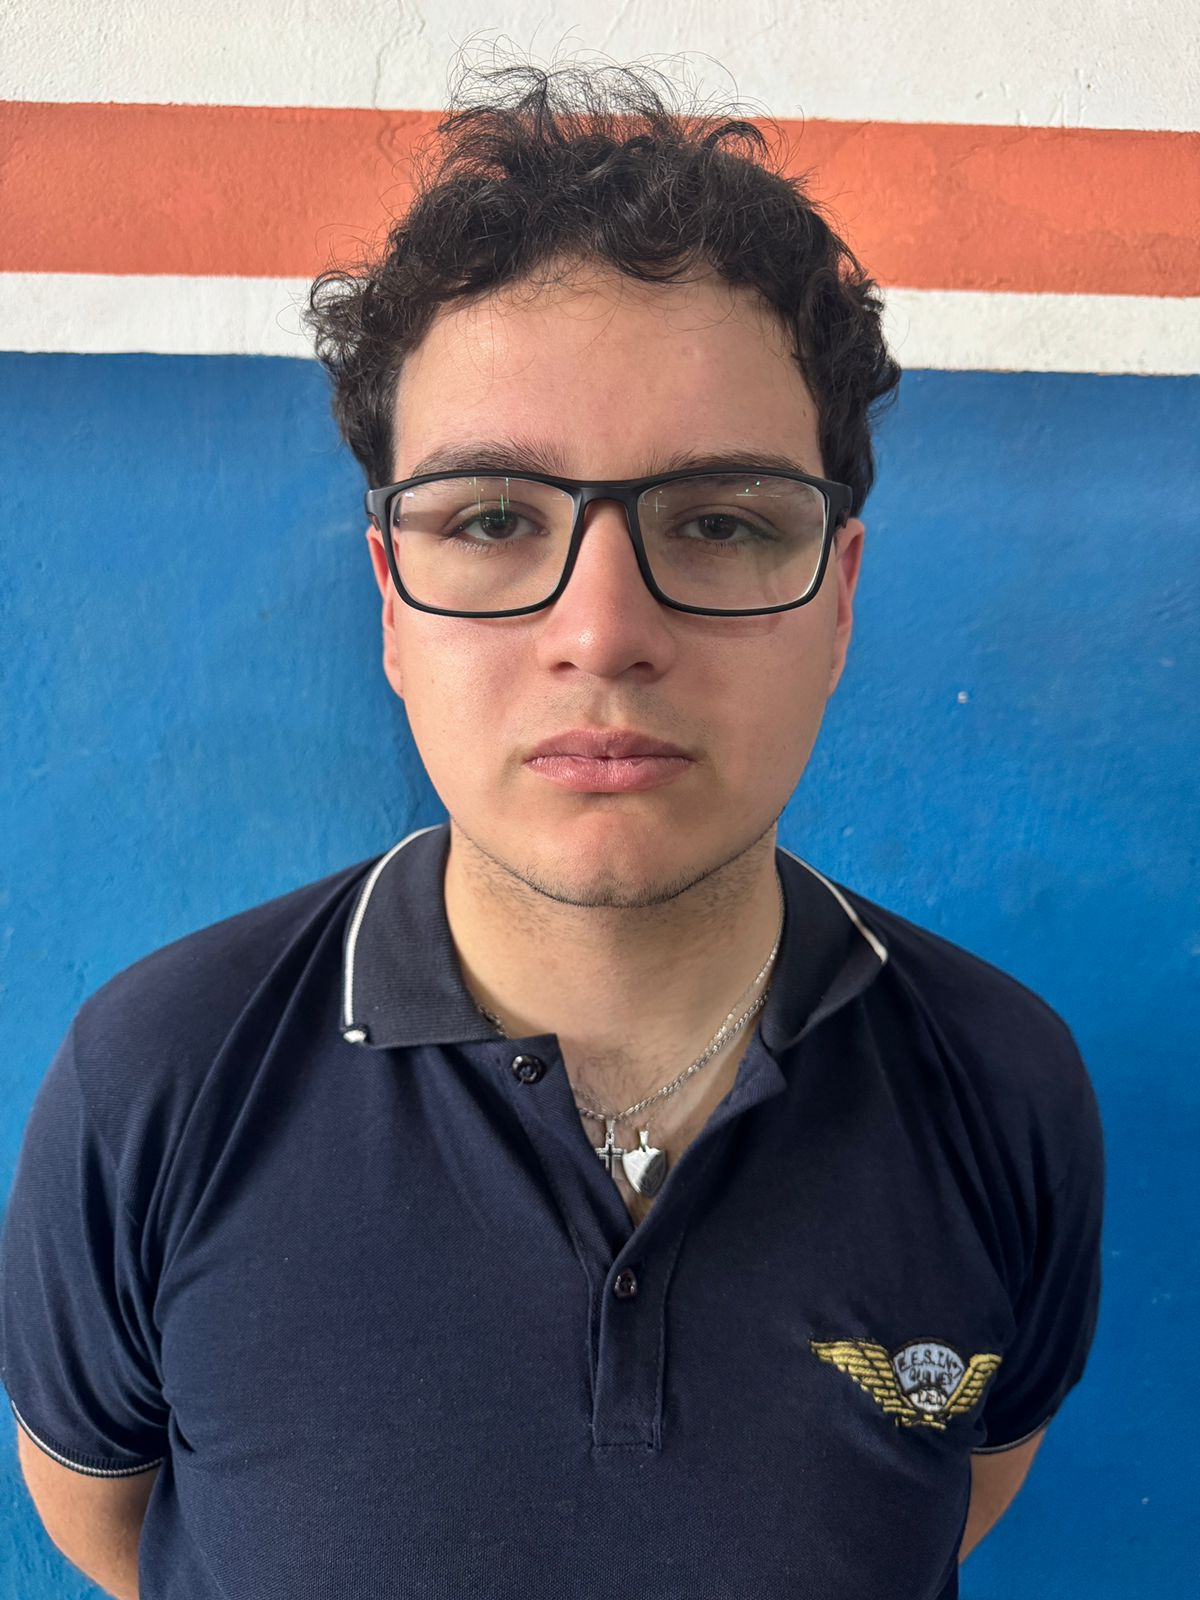
\includegraphics[width=0.4\linewidth]{Carpeta tecnica/Fotoramiro.jpg}
\end{figure}
\begin{center}
Castillo Ramiro\\
DNI: 47516171\\
7°2 Aviónica
\end{center}

\begin{figure}[H]
    \centering
    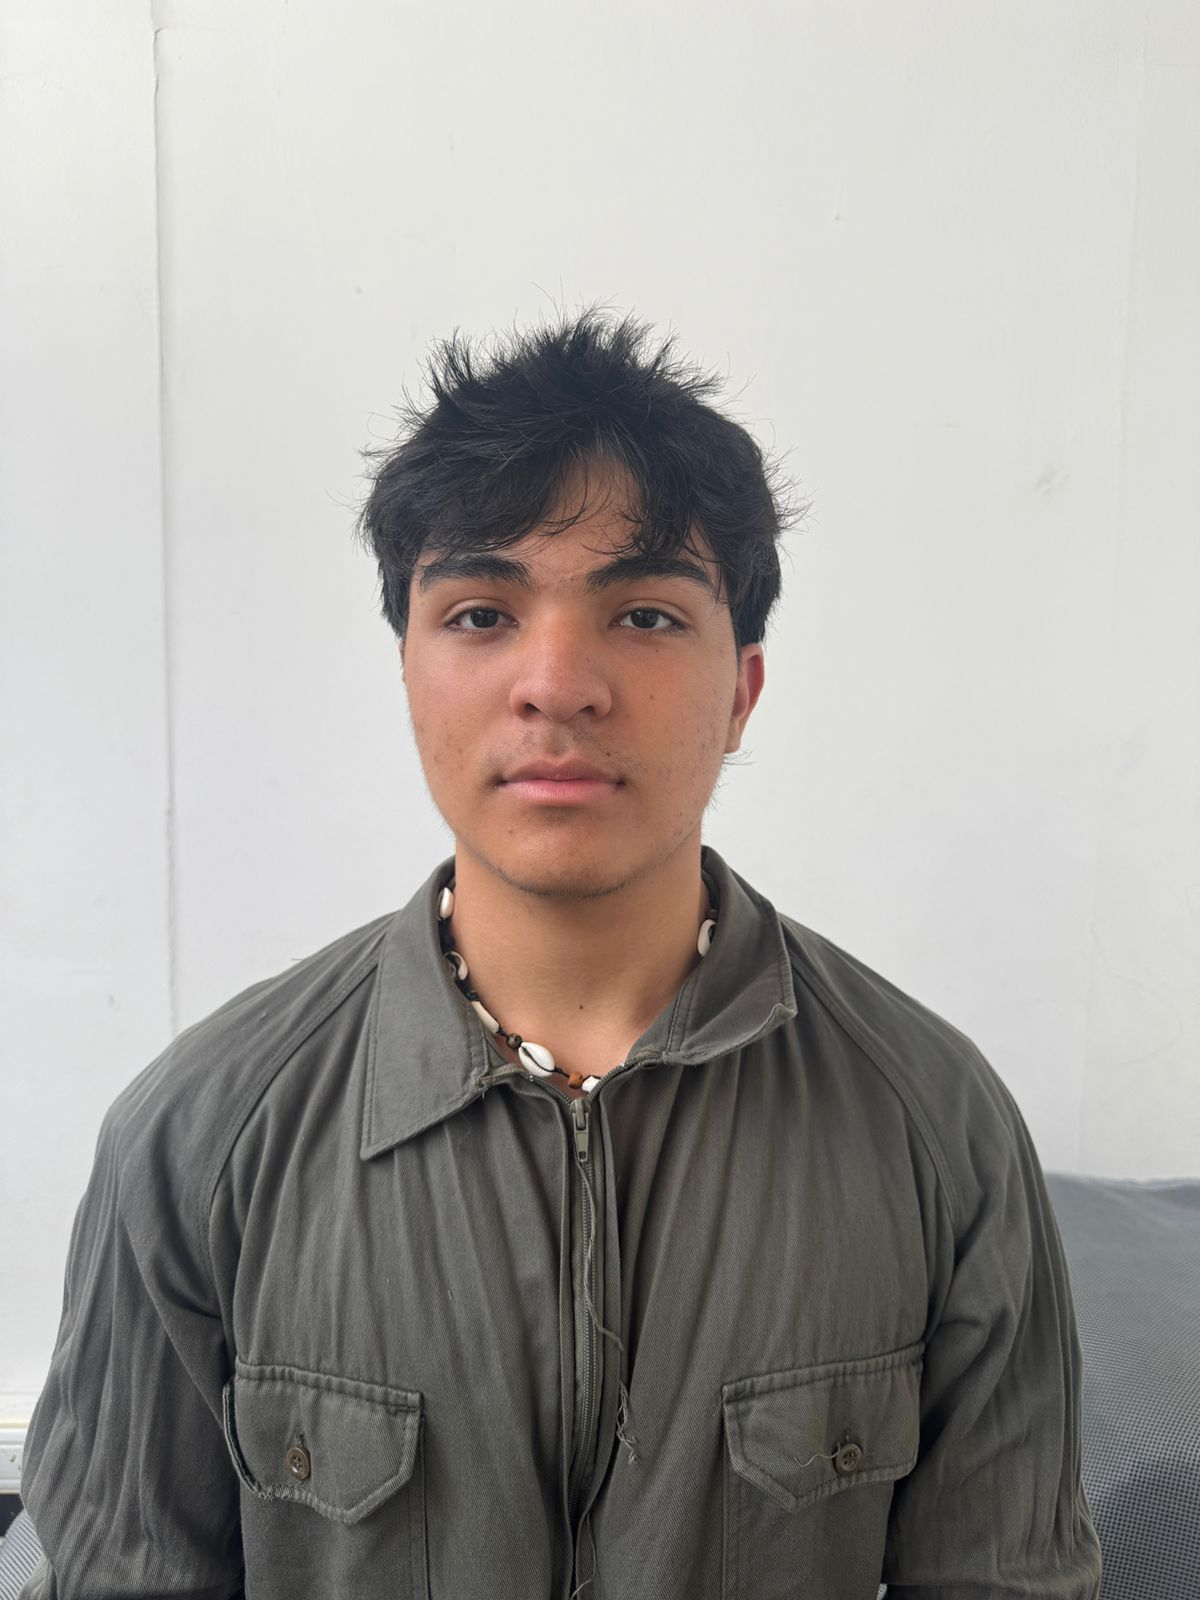
\includegraphics[width=0.4\linewidth]{Carpeta tecnica/fotopino.jpg}
\end{figure}
\begin{center}

Pino Octavio\\
DNI: 47882634\\
7°2 Aviónica
\end{center}

\begin{figure}[H]
    \centering
    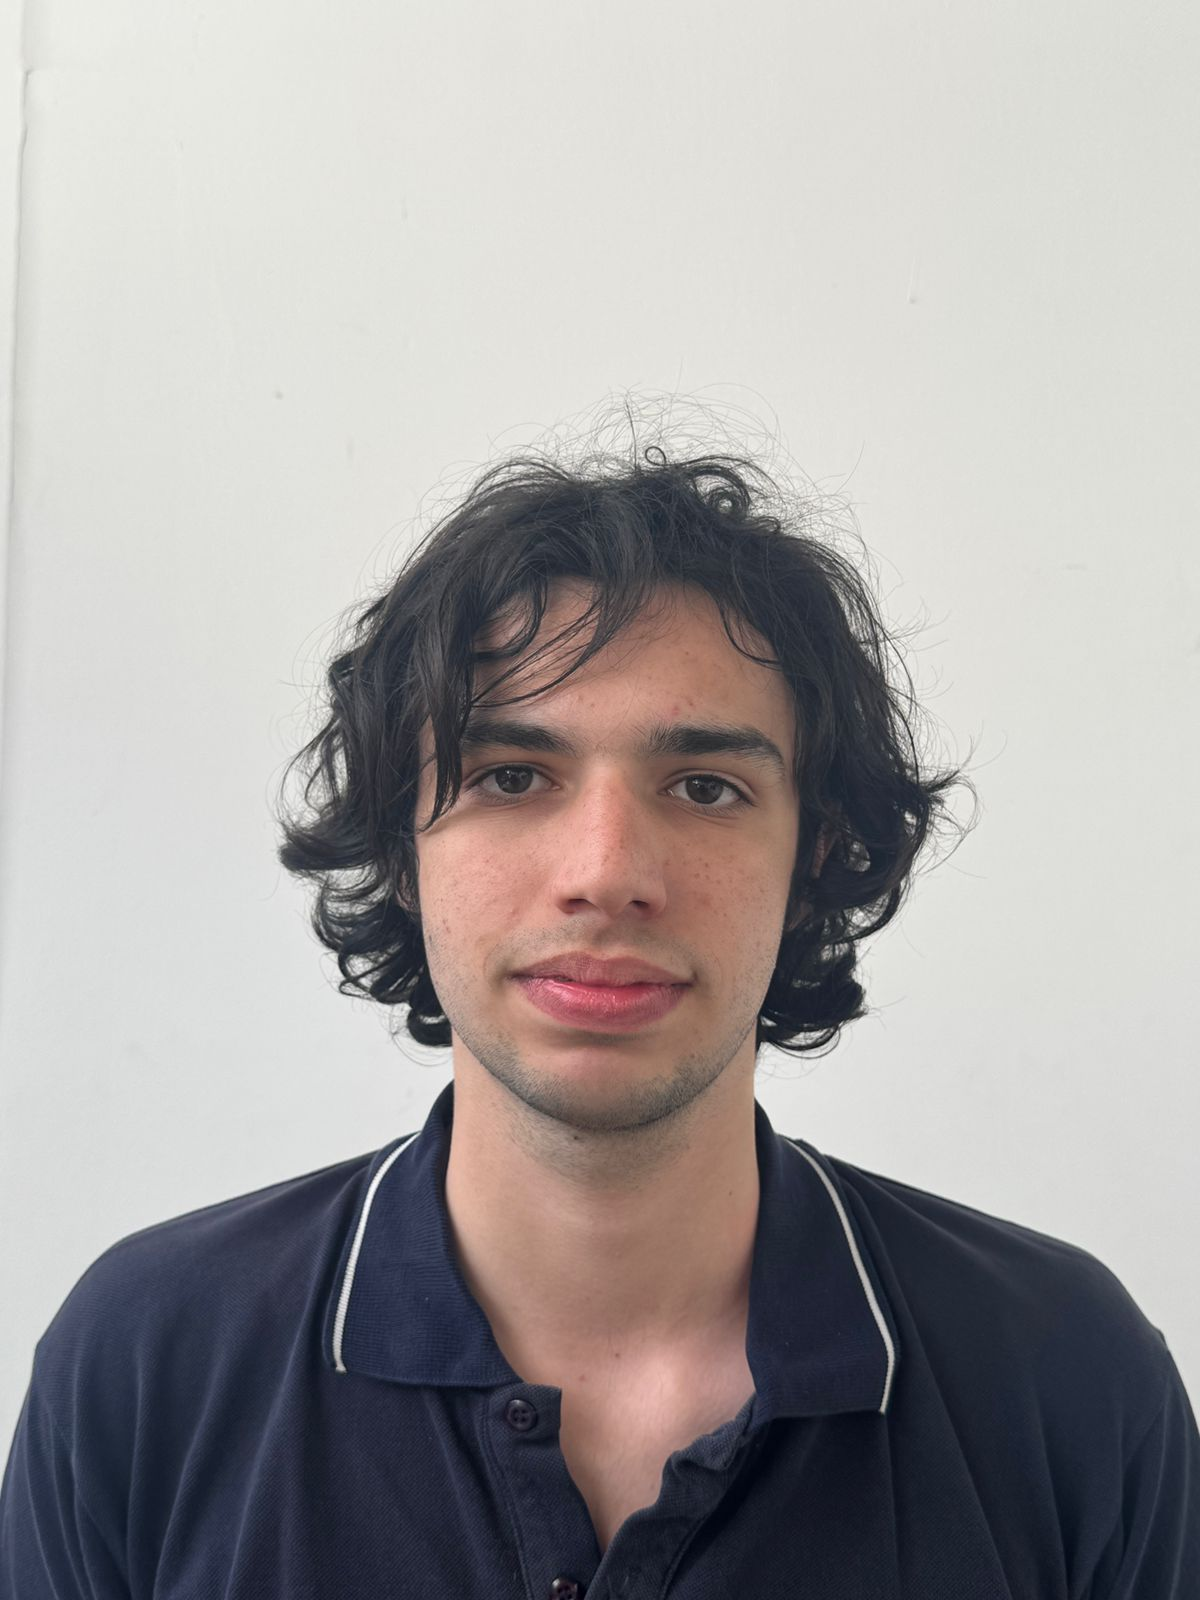
\includegraphics[width=0.4\linewidth]{Carpeta tecnica/Fototiago.jpg}
\end{figure}

\begin{center}
Quattrocchi Tiago\\
DNI: 47510542\\
7°2 Aviónica
\end{center}

\begin{figure}[H]
    \centering
    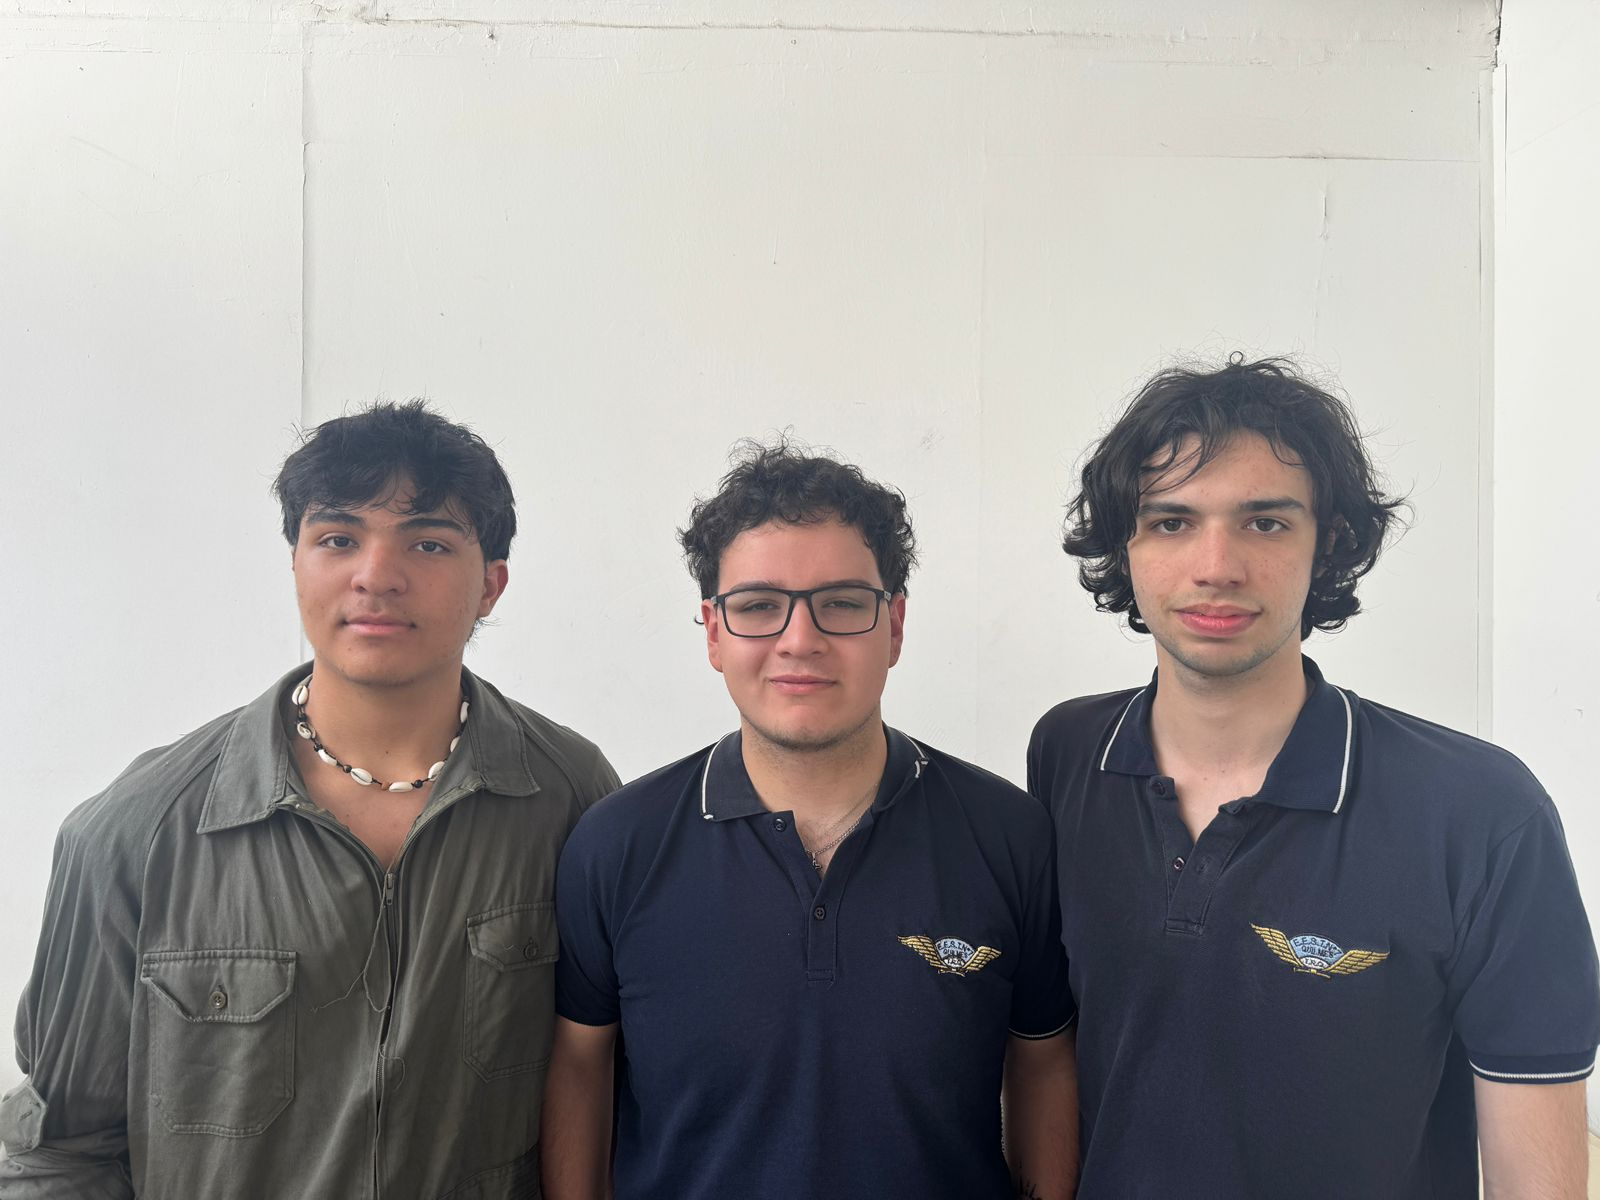
\includegraphics[width=0.7\linewidth]{Carpeta tecnica/Fotogrupo.jpg}
    \caption{Grupo BlindAssist}
\end{figure}

\subsection{Docentes a Cargo}
    \begin{center}
        \begin{itemize}
        \item Argüello Gabriel
        \item Bianco Carlos
        \item Carlassara Fabrizio
        \item Medina Sergio
        \item Palmieri Diego
        \end{itemize}
    \end{center}

\subsection{Desarrollo del proyecto}
\subsubsection*{Fecha de Inicio}
14/4/2025
\subsubsection*{Duración del proyecto}
25 Semanas
\subsubsection*{Esfuerzo del proyecto}
Maximo de 8 horas de trabajo (200 horas de trabajo en todo el año)
\subsubsection*{Lenguajes utilizados}
\begin{itemize}
\item LaTex
\item CSS
\item HTML
\item Python
\item Javascript
\end{itemize}

\subsubsection*{Programas utilizados}

\begin{itemize}
    \item OverLeaf
    \item Visual Studio Code
    \item Github Desktop
    \item Termius
    \item Proteus 8
    \item AutoCad
    \item UltiMaker
    \item Benewake Software
\end{itemize}

\section{Descripción}

\subsection{Objetivo}
El objetivo de este proyecto es mantener la integridad de las personas ciegas o con algún tipo de discapacidad visual en cualquier tipo de entorno urbano y darles un mayor nivel de conciencia en entornos mas cerrados. Para ello, desarrollamos un dispositivo que mediante reconocimiento por inteligencia artificial y la detección de objetos utilizando tecnología láser para avisar al usuario sobre un obstáculo en frente, por encima de la cadera, la presencia de alguna persona en un espacio cerrado y la cantidad de individuos que se encuentran en el mismo espacio, contando con alertas sonoras y vibratorias que no alteren su percepción y condición actual.Este dispositivo funcionara como una ayuda al bastón que utilizan en su día a día sin modificar su efectividad o tratar de reemplazar su función.

\subsection{Alcance}
\begin{itemize}

\item Cómo objetivo final, querríamos que este este proyecto llegue a ser un prototipo funcional y autónomo, con el menor tamaño posible para la comodidad del usuario. Contar con una IA correctamente entrenada y optimizada en rendimiento, que trabaje en conjunto al área cubierta y sensada por los lasers. Teniendo en cuenta las posibilidades, buscamos que las alertas sensoriales sean claras para el usuario así tiene una experiencia placentera en su día a día.
\end{itemize}

\subsection{Temática}

 \begin{itemize}
 \item Inclusión social: Nuestro proyecto abarca los parámetros presentados en la temática de inclusión social. Esto debido a que el proyecto mismo busca ayudar con el tránsito de las personas con discapacidad tanto en la vía pública cómo lugares cerrados desconocidos. Además, también puede ayudar con su comunicación y vida social, ya que los alerta de las personas que tienen a su alrededor. 
 \end{itemize}
 
\subsection{Problemas a resolver}

\begin{itemize}
\item Obstáculos repentinos en la vía publica, pueden presentar dificultad a la hora de detectar postes, árboles y otros peligros inesperados que se encuentren por encima de su tren inferior (a partir de la cadera), siendo que la mayoría de las veces el rango que cubre el bastón no es suficiente para detectar y avisar efectivamente a la persona con discapacidad visual.
\item El riesgo constante que sufren en la vía publica termina llevando a que dependan mucho de terceros, como puede ser transeúntes que los apoyen o en casos de personas con una edad mas avanzada, un cuidador designado o familiar cercano. Tenemos en cuenta la falta de autonomía que genera esta problemática, la dependencia que terminan teniendo de terceros es una de las problemáticas más importantes a resolver y la idea es darles una herramienta de autonomía e integración.
\item Proteger su intimidad pudiendo detectar personas que están en el mismo espacio cerrado sin depender de que la persona avise de su llegada, también permitiéndoles conocer la ubicación de dichos individuos, dándole un mejor sentido y conciencia situacional.
\end{itemize}

\subsection{Público beneficiado}
El proyecto está destinado a personas con impedimentos visuales. En el mundo hay 2200 millones de personas con visibilidad reducida, 43,3 millones son no videntes. Esta es la demográfica que será beneficiada directamente por el proyecto, habilitando el tránsito por la vía pública de manera más segura y sin problemas que puedan llegar a afectar su integridad o la rehabilitación a la que están sometidos. Además, al ser un accesorio portable, compacto y difícil de perder u olvidar, no interrumpe en las acciones que pueda realizar el usuario en su vida cotidiana. Este proyecto también beneficiará indirectamente a instituciones privadas como seguros de salud y ART (Aseguradoras de Riesgo del Trabajo), ya que estos pueden ofrecerle como una ayuda al grupo de personas antes descritas. También aplica para la vida cotidiana o la vida pública, ya que se reduce el riesgo de accidentes y la carga que supone a los familiares a la hora de ayudarlo.



\begin{figure}[H]
    \centering
    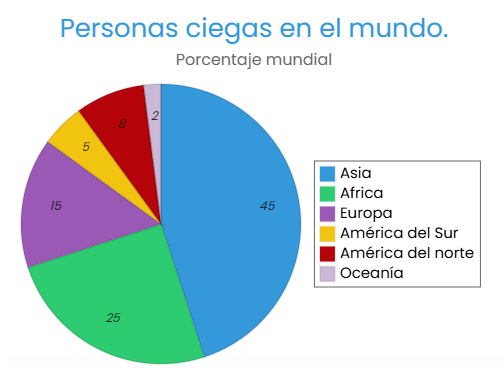
\includegraphics[width=0.8\linewidth]{Carpeta tecnica/graf1.png}
    \caption{Tabla de población ciega por continentes.}
\end{figure}

\subsection{Impacto}
 \begin{itemize}
 
\item En un contexto social, este prototipo tiene el potencial de transformar la vida de millones de personas. Como mencionamos anteriormente, más de 40 millones de personas en todo el mundo viven con discapacidad visual. Este impacto no solo afectaría a las personas con esta discapacidad, sino también a sus cuidadores y familiares directos. Es decir, podría beneficiar a una gran cantidad de personas y comunidades. Especialmente en regiones como África, Asia y América del Sur, donde existe un alto número de personas con discapacidad visual, pero donde los recursos y la infraestructura necesarios para facilitar su movilidad y vida cotidiana son limitados.

     
 \end{itemize}

\subsection{Descripción General}

\begin{itemize}

    \item BlindAssist es un proyecto que busca facilitar el tránsito de sus usuarios en la vida cotidiana. A través de un dispositivo colgante que puedan llevar encima mismos o en algún accesorio que mejore su movilidad. Esto lo lograríamos con un conjunto de componentes que trabajan en coordinación. Primero una cámara que detecta elementos específicos, por poner un ejemplo: cestos de basura, señalizaciones, etc. Segundo, unos sensores láser que detectan la proximidad de obstáculos cómo ramas u postes. Cómo tercero, alertas sensoriales a través de audio y vibraciones para alertar al usuario y que este pueda evitar estos inconvenientes.
    
\end{itemize}

\subsection{Funcionalidades}
\begin{itemize}
    \item El dispositivo presenta dos etapas de detección y dos de alerta al usuario. 
    El dispositivo realizará mediciones de distancia mediante los sensores TFmini LIDAR, estos se encuentran dispuestos de tal forma que puedan cubrir varios ángulos en frente de la persona. Acorde a la detección de los sensores, se le comunica al usuario la posición de un objeto intruso en el rango frontal, dependiendo que sensores detectan un objeto a menor distancia que 120cm se realizara un control de potencia de los motores internos, hay dos motores de vibración, uno a la izquierda y derecha del dispositivo, cada uno acorde a los sensores LIDAR de ambos lados, Cuando se detecta algo en el tercer TFmini cambia la organización, ambos motores emitirán la misma potencia, en caso de que el motor frontal y lateral detecten algo dicho lado tendrá un control titilante de la vibración, en caso de que los tres sensores se activen, ambos motores vibran al máximo de potencia.\\
    El sistema de detección basado en Inteligencia Artificial (IA), utiliza la cámara para capturar imágenes continuamente. Un modelo de IA avanzado (YOLOv8) actúa como el cerebro, escaneando cada imagen a alta velocidad para identificar y clasificar objetos relevantes para la seguridad, como personas, autos, bicicletas, camiones y objetos de tropiezo (botellas, etc.). Solo se anuncia un objeto si la IA está lo suficientemente segura de su clasificación (más del 60\% de confianza).
    La comunicación se realiza mediante voz asíncrona. Esta es la clave de la velocidad: el mensaje de voz (``Una persona", "3 autos", "Moto fuera") se envía a un proceso en segundo plano, permitiendo que la cámara y la IA sigan escaneando el entorno sin detenerse ni un instante. Para evitar el ruido constante, un filtro de tiempo de espera (cooldown) asegura que solo se anuncien los cambios de estado (algo nuevo apareció, se fue o cambió de cantidad) y no se repita la misma alerta cada pocos segundos.
    
\end{itemize}

\separador

%--- Hardware ---
\section{Hardware}

\subsection{Raspberry Pi 4}
La Raspberry Pi 4 es una computadora de placa única (SBC) compacta y de bajo consumo que sirve como el "cerebro" de su proyecto. A diferencia de las computadoras de escritorio tradicionales, está diseñada para tareas especializadas y prototipado. Utiliza un procesador Broadcom BCM2711 de cuatro núcleos y una arquitectura ARM, lo que la hace ideal para aplicaciones de robótica y automatización. Su funcionamiento se basa en la ejecución de un sistema operativo, como Raspberry Pi OS, que permite programar y controlar los componentes conectados a sus pines de GPIO (General Purpose Input/Output).
\begin{figure}[H]
\centering
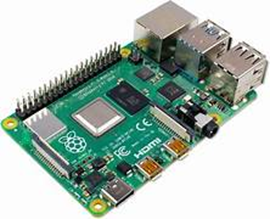
\includegraphics[width=0.5\linewidth]{Carpeta tecnica/Imagen2.png}
\caption{Modulo Raspberry PI 4}
\end{figure}

\subsubsection{PWM}

El PWM (Pulse Width Modulation) en la Raspberry Pi 4 es una técnica digital para generar señales moduladas en ancho de pulso que permiten controlar la potencia aplicada a dispositivos electrónicos.
En este modelo de placa, el PWM puede implementarse tanto por hardware (pines GPIO dedicados) como por software (emulación mediante librerías como RPi.GPIO o pigpio).

\begin{figure}[H]
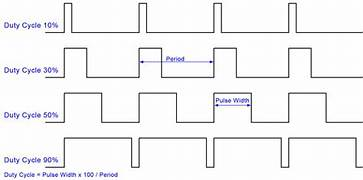
\includegraphics[width=0.9\linewidth]{Carpeta tecnica/PWM.png}
\caption{Duty cicle de PWM}
\end{figure}

\paragraph{Funcionamiento}
El PWM consiste en la generación de una onda cuadrada con dos parámetros principales:

\begin{itemize}
\item Frecuencia (f): cantidad de ciclos por segundo (Hz).

\item Duty cycle (\%): proporción del tiempo en que la señal está en estado alto respecto del periodo total.

La potencia media entregada a la carga es proporcional al duty cycle.
\end{itemize}

Ejemplo:

\begin{itemize}
\item 0\% duty → salida siempre en nivel bajo (0 V).

\item 50\% duty → salida mitad del tiempo en nivel alto.

\item 100\% duty → salida siempre en nivel alto (3,3 V en GPIO).
\end{itemize}

\paragraph{Pines PWM en Raspberry Pi 4}

La Raspberry Pi 4 posee 2 canales PWM de hardware, cada uno con salidas asignables a diferentes GPIO según la configuración.
Algunos pines disponibles:

\begin{itemize}

\item Canal PWM0: GPIO 12 (pin 32), GPIO 18 (pin 12).

\item Canal PWM1: GPIO 13 (pin 33), GPIO 19 (pin 35).

\end{itemize}

\subsubsection{UART}

El UART (Universal Asynchronous Receiver-Transmitter) es un protocolo de comunicación serie asíncrono que transmite y recibe datos bit a bit mediante dos líneas:

\begin{itemize}
    
\item TX (Transmit): envía datos.

\item RX (Receive): recibe datos.

\end{itemize}

\begin{figure} [H]
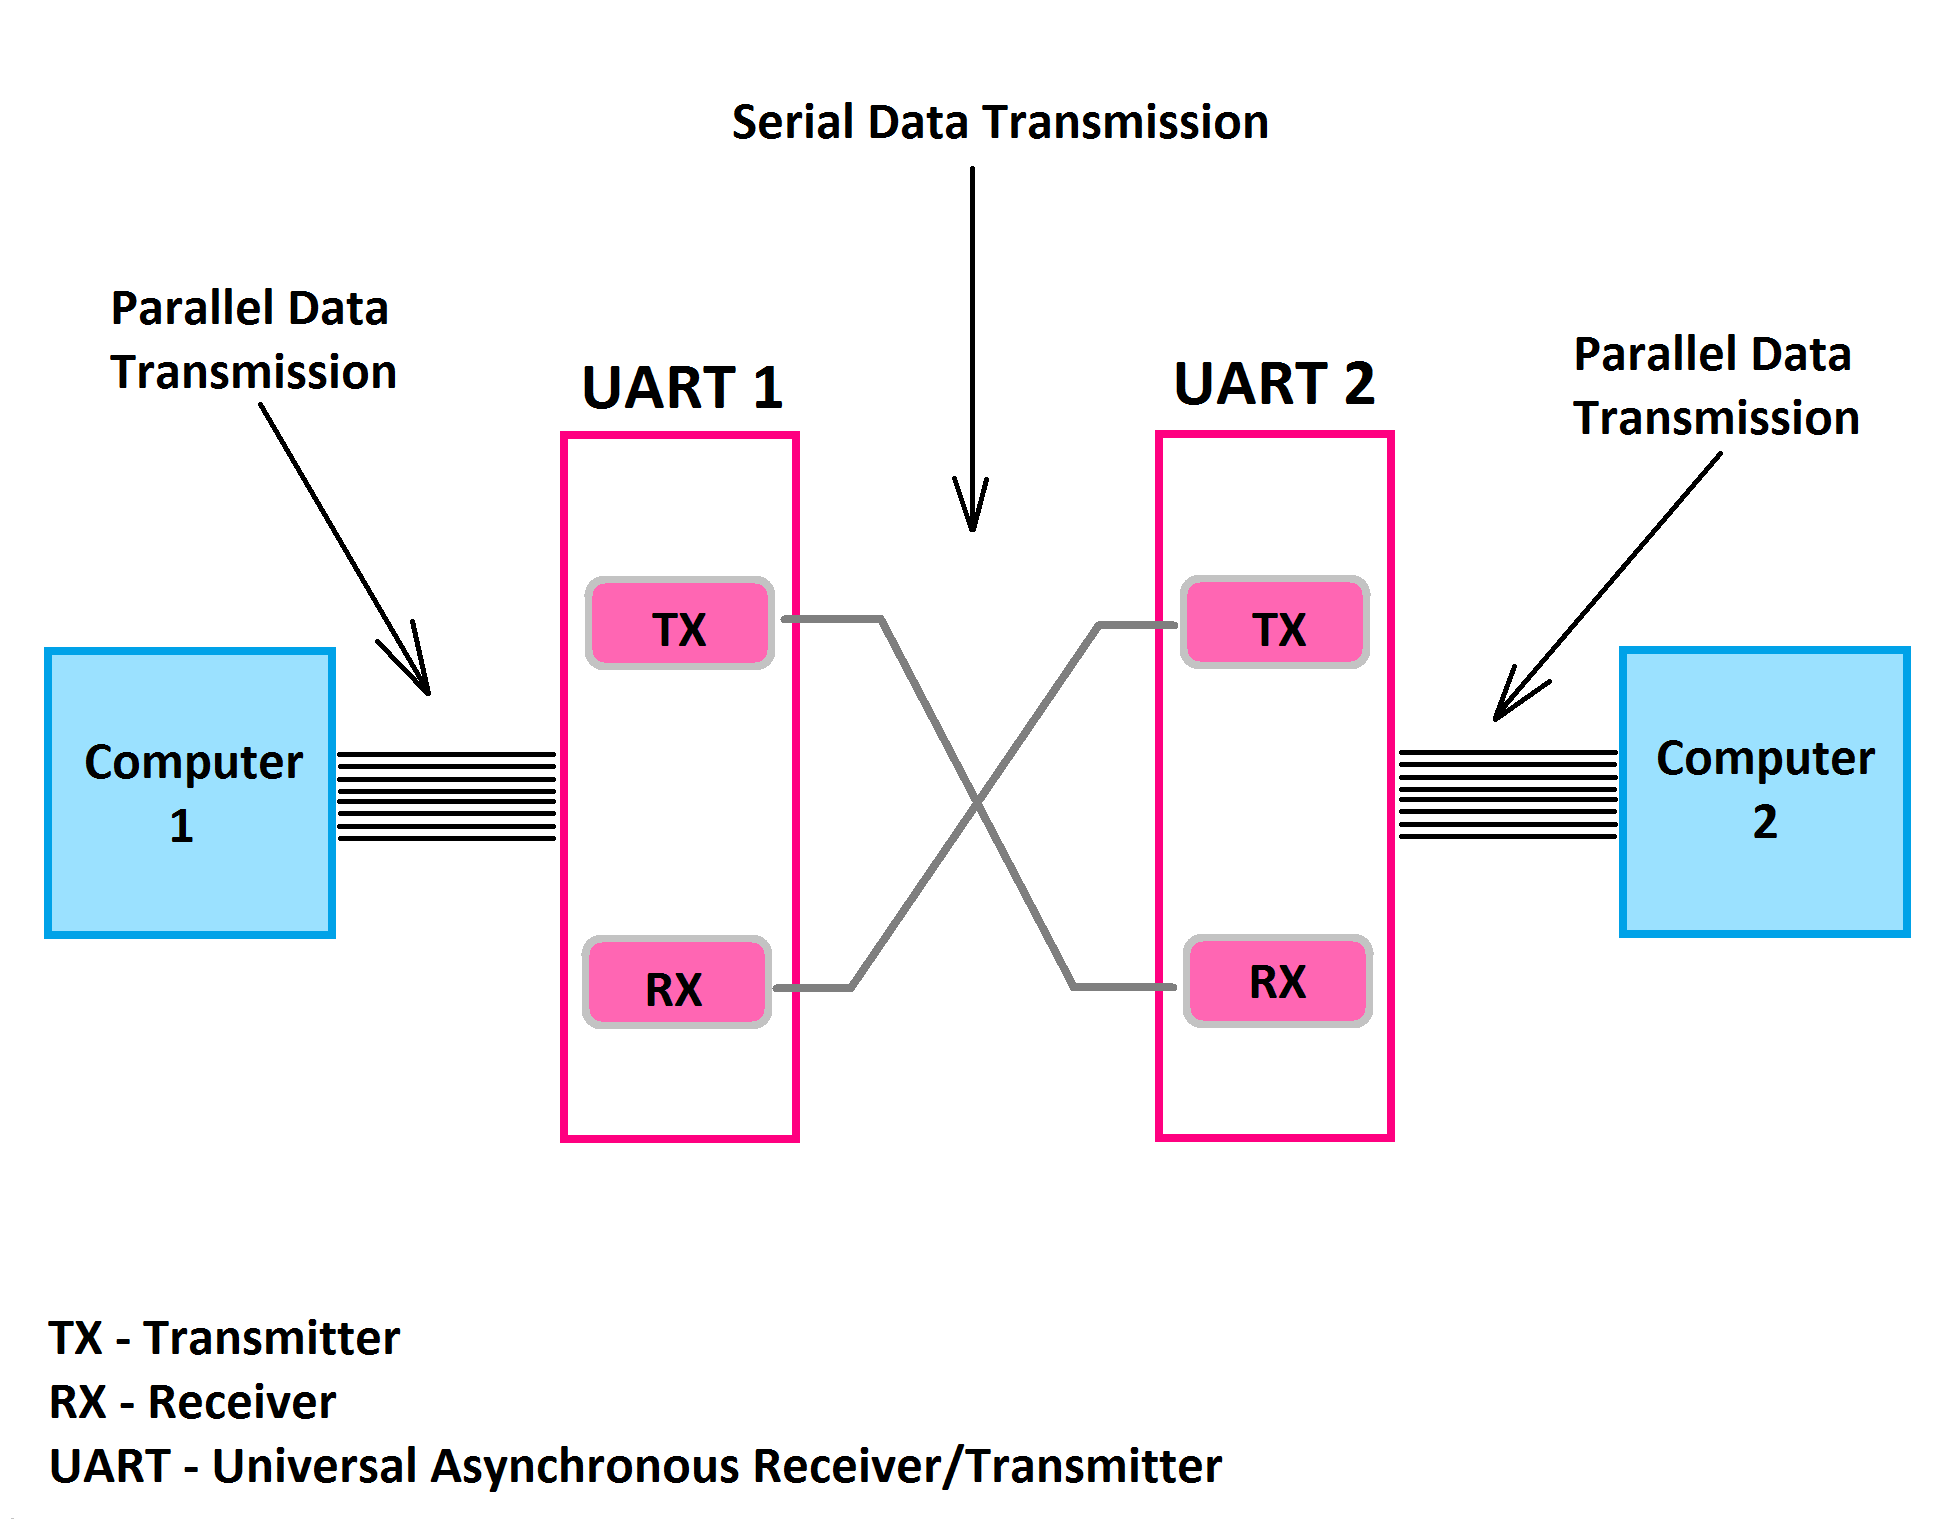
\includegraphics[width=0.9\linewidth]{Carpeta tecnica/Conexion UART.png}
\caption{Conección UART}
\end{figure}

En la Raspberry Pi 4, el UART permite la comunicación directa con módulos, microcontroladores, sensores y periféricos externos, usando niveles lógicos de 3,3 V.

\paragraph{Funcionamiento}

La transmisión UART se basa en una trama de datos que incluye:

\begin{itemize}
\item Bit de inicio (Start bit).

\item Datos (5 a 8 bits).

\item Bit de paridad (opcional).

\item Bit(es) de parada (Stop bit).
\end{itemize}

\begin{figure}[H]
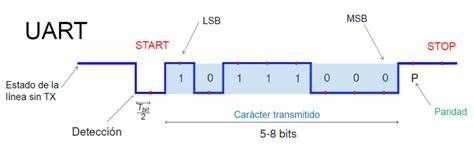
\includegraphics[width=\linewidth]{Carpeta tecnica/UART.png}
\caption{Transmisión de Bits en UART}
\end{figure}

El reloj no se transmite; la sincronización se logra configurando ambas partes con la misma tasa de baudios (baud rate), por ejemplo 9600, 115200 bps.

Es asíncrono, no requiere señal de reloj adicional como en SPI o I²C.

\paragraph{UARTs disponibles en Raspberry Pi 4}

La placa incluye varios controladores UART, aunque no todos están habilitados de forma predeterminada:

\begin{itemize}
\item PL011 (UART principal): más robusto, configurable. Por defecto está mapeado en los pines GPIO14 (TX) y GPIO15 (RX).

\item Mini UART: secundario, con funciones más limitadas.
\end{itemize}

Pines UART por defecto (GPIO – Raspberry Pi 4):

\begin{itemize}
\item GPIO14 (TXD0) → Pin físico 8

\item GPIO15 (RXD0) → Pin físico 10
\end{itemize}

\subsubsection{Esquemático}
\begin{figure}[H]
    \centering
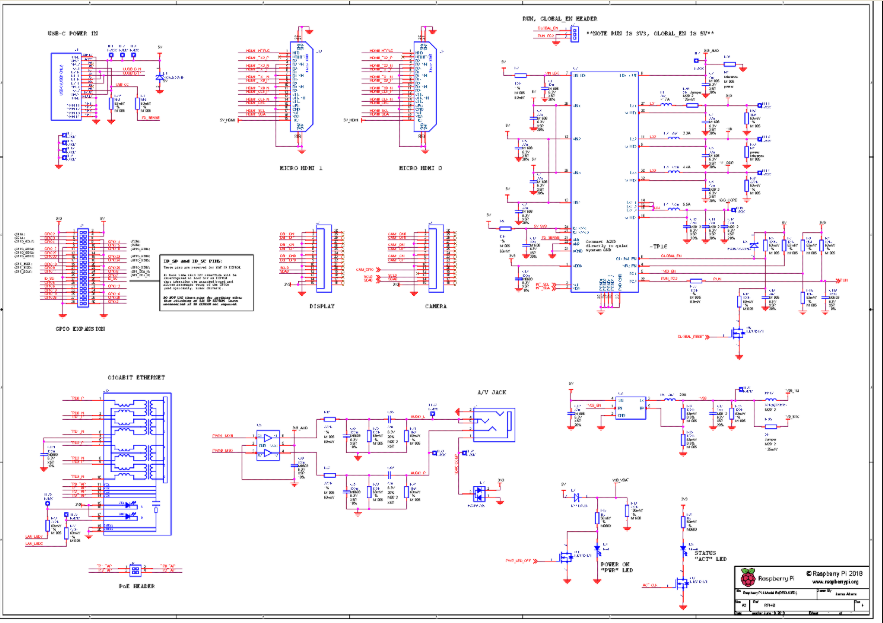
\includegraphics[width=0.9\linewidth]{Carpeta tecnica/Esquematico Raspberry.png}
\caption{Esquematico de la Raspberry PI 4}
\end{figure}

\subsubsection{Pinout}
\begin{figure}[H]
    \centering
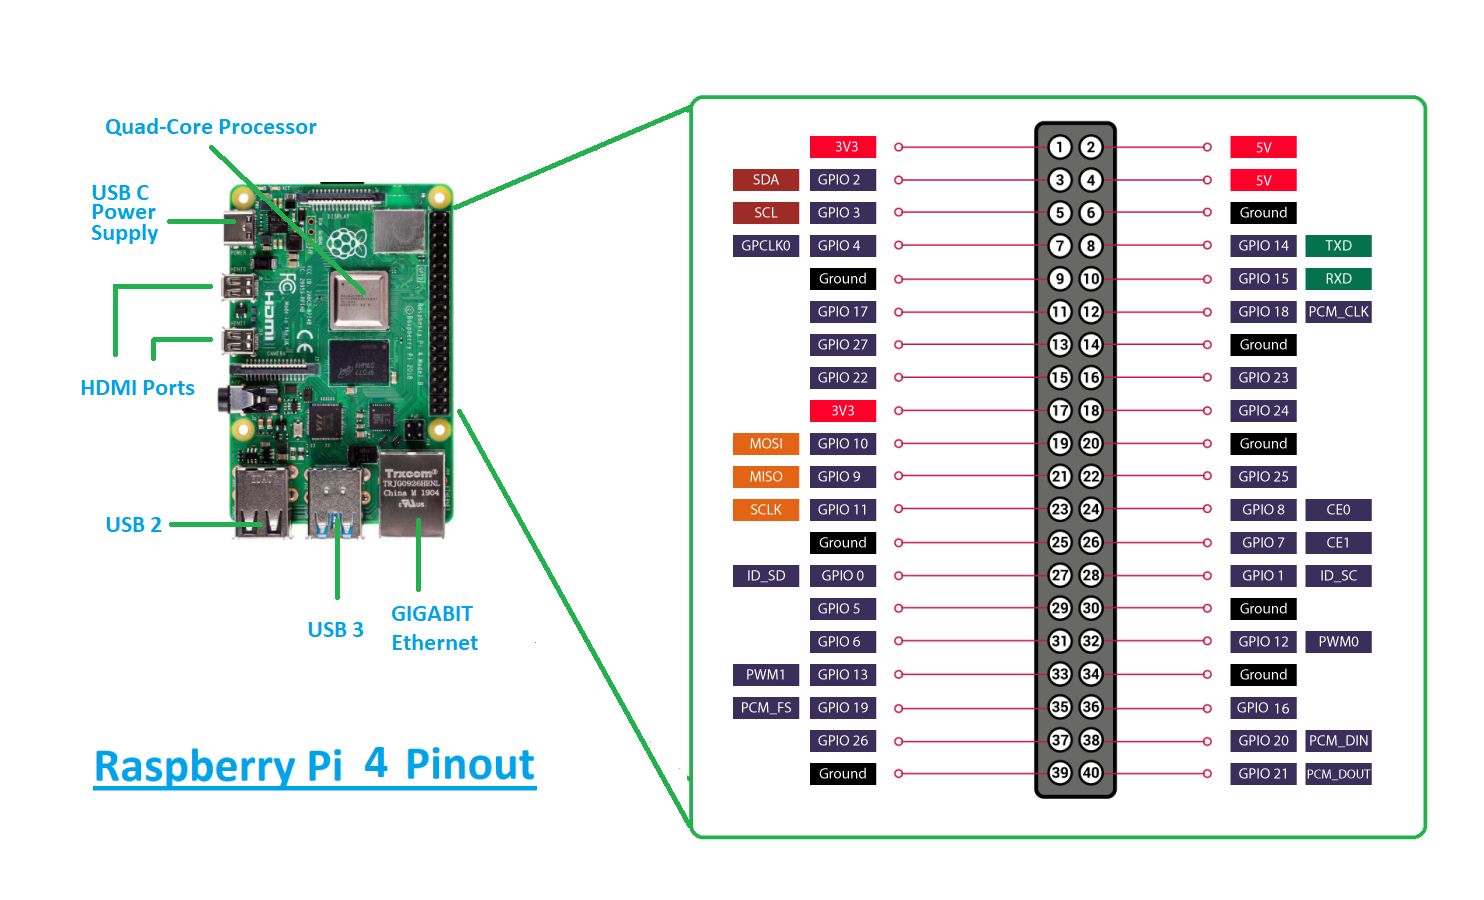
\includegraphics[width=\linewidth]{Carpeta tecnica/Pinout4.png}
\caption{Pinout de la Raspberry PI4}
\end{figure}

\subsection{Raspberry PI CAM V1.3}

\begin{figure}[H]
    \centering
    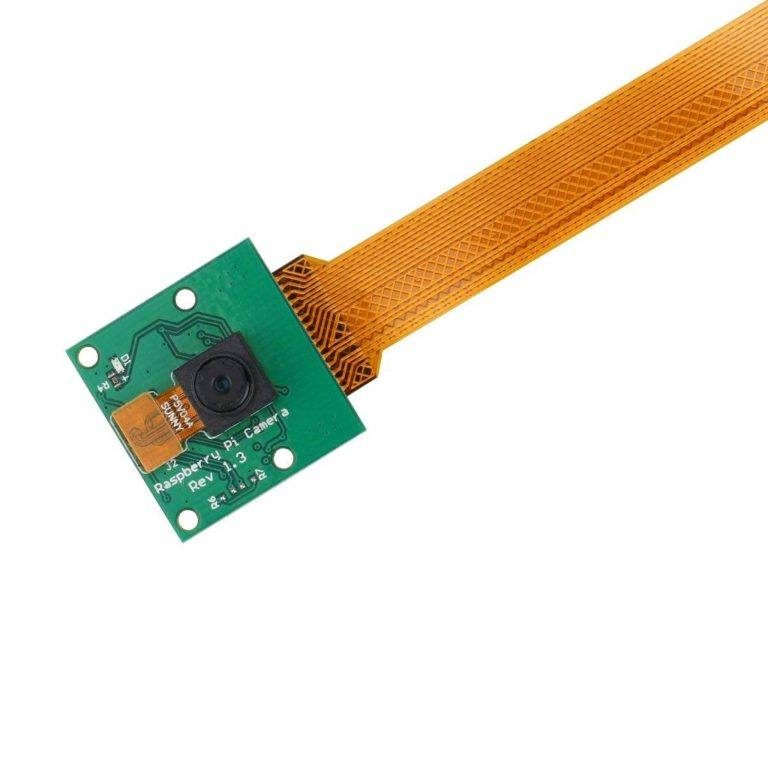
\includegraphics[width=0.5\linewidth]{Carpeta tecnica/berrycam.png}
    \caption{Raspberry PI CAM V1.3}
\end{figure}

La Raspberry Pi Camera Module v1.3 es una cámara oficial diseñada para las placas Raspberry Pi, basada en el sensor OmniVision OV5647 de 5 megapíxeles. Permite capturar imágenes fijas de hasta 2592×1944 píxeles y grabar video en resoluciones de 1080p a 30 fps, 720p a 60 fps y 480p a 90 fps. Se conecta mediante un cable plano CSI (Camera Serial Interface), lo que asegura una transmisión de datos rápida y optimizada.

Este módulo es compacto y ligero, ideal para visión por computadora, robótica, monitoreo y aplicaciones de IoT. Gracias a su integración directa con la Raspberry Pi y la compatibilidad con librerías como Picamera y OpenCV.

\subsubsection{Tablas de parametros}

\begin{table}[H]
\begin{tabular}{|p{4cm}|p{11cm}|}
\hline
\textbf{Parámetro} & \textbf{Descripción} \\ \hline
Tipo de sensor & OmniVision OV5647 Color CMOS QSXGA (5 megapíxeles). \\ \hline
Tamaño del sensor & 3,67 x 2,74 mm. \\ \hline
Contenido de píxeles & 2592 x 1944 píxeles. \\ \hline
Tamaño de píxel & 1,4 x 1,4 µm. \\ \hline
Tamaño de la placa & 25 x 24 mm (sin cable flexible). \\ \hline
\end{tabular}
\caption{Tabla de especificaciones técnicas}
\end{table}

\begin{table}[H]
\begin{tabular}{|p{4cm}|p{11cm}|}
\hline
\textbf{Parámetro} & \textbf{Descripción} \\ \hline
Objetivo & f = 3,6 mm. \\ \hline
Abertura & f/2,9. \\ \hline
Longitud focal & 3,29 mm. \\ \hline
Ángulo de visión & 54° (horizontal) x 41° (vertical). \\ \hline
Campo de visión total & 72,4°. \\ \hline
Campo de visión a 2 m & 2,0 x 1,33 m. \\ \hline
Equivalencia & Lente SLR de 35 mm en formato completo. \\ \hline
Enfoque & Fijo, desde 1 m hasta infinito. \\ \hline
\end{tabular}
\caption{Tabla de parámetros ópticos}
\end{table}

\subsubsection{Rendimiento Fotográfico}
\begin{table}[H]
\begin{tabular}{|p{4cm}|p{11cm}|}
\hline
\textbf{Parámetro} & \textbf{Descripción} \\ \hline
Disparo mínimo & 1/4 s a 5 m. \\ \hline
Resolución de imagen fija & Hasta 2592 x 1944 px (5 MP). \\ \hline
\end{tabular}
\caption{Tabla de rendimiento fotográfico}
\end{table}

\begin{table}[H]
\begin{tabular}{|p{4cm}|p{11cm}|}
\hline
\textbf{Parámetro} & \textbf{Descripción} \\ \hline
Vídeo Full HD & 1080p a 30 fps (códec H.264/AVC). \\ \hline
Vídeo HD & 720p a 60 fps. \\ \hline
Vídeo VGA & Hasta 90 fps. \\ \hline
\end{tabular}
\caption{Tabla de rendimiento de video}
\end{table}

\subsection{TFmini}
El TFmini es un sensor de distancia LiDAR (Light Detection and Ranging). Funciona emitiendo un pulso de láser infrarrojo y midiendo el tiempo que tarda la luz en rebotar en un objeto y regresar al sensor. Esta técnica, conocida como tiempo de vuelo (ToF), le permite calcular la distancia con precisión. Se comunica con la Raspberry Pi a través de interfaces como UART (puerto serie) o I2C, lo que le permite obtener lecturas de distancia de forma rápida y confiable.

\begin{figure}[H]
    \centering
    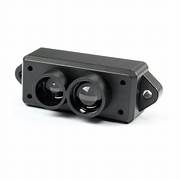
\includegraphics[width=0.5\linewidth]{Carpeta tecnica/TFmini.png}
    \caption{TFmini S}
\end{figure}

\subsubsection{Descripción General y Principio de Funcionamiento}

El TFmini es un mini módulo LiDAR diseñado para realizar funciones de medición de distancia sin contacto y en tiempo real. Se caracteriza por ofrecer una medición de distancia precisa, estable y de alta velocidad.

El sensor opera bajo el principio de TOF (Time of Flight). El módulo transmite periódicamente una onda de modulación de rayo infrarrojo cercano que se refleja al contactar un objeto. El producto calcula el rango relativo al objeto al medir la diferencia de fase de ida y vuelta (tiempo de vuelo) de la señal.

\begin{figure}[H]
    \centering
    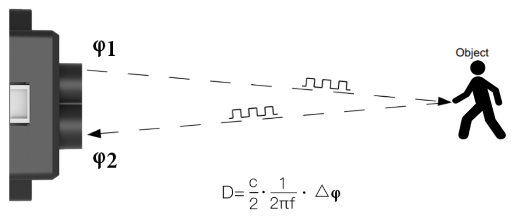
\includegraphics[width=0.8\linewidth]{Carpeta tecnica/principvuelo.png}
    \caption{Principio de tiempo de vuelo}
    \label{fig:placeholder}
\end{figure}

\subsubsection{Tablas de parametros}

\begin{table}[H]
\centering
\begin{tabular}{|p{5cm}|p{5cm}|p{5cm}|}
\hline
\textbf{Característica} & \textbf{Parámetro} & \textbf{Notas} \\
\hline
Rango de Operación (Interior) & 0.3 m -- 12 m & Alcance máximo bajo condiciones de interior y pizarra blanca estándar (reflectividad del 90\%). \\
\hline
Precisión de Medición & $\pm 6$ cm (@ 0.3 m - 6 m) / $\pm 1\%$ (@ 6 m - 12 m) &  \\
\hline
Frecuencia (Tasa de Salida) & 100 Hz & Una salida de datos cada 10 ms. \\
\hline
Resolución de Rango & 1 cm &  \\
\hline
Unidad de Distancia por Defecto & cm (centímetros) & Se puede modificar a mm (milímetros) mediante instrucción. \\
\hline
Zona Ciega de Detección & 0 - 30 cm & Los datos en este rango no se consideran fiables. \\
\hline
Ángulo Medio de Recepción ($\beta$) & 1.15° &  \\
\hline
Ángulo Medio de Transmisión & 1.5° &  \\
\hline
\end{tabular}
\caption{Tabla de parámetros y rendimiento}
\end{table}

El rango puede verse afectado por la intensidad de la iluminación ambiental y la reflectividad del objeto. Por ejemplo, en condiciones de deslumbramiento extremo (exterior a mediodía de verano, $\approx 100$ klux) y detección de un objetivo negro (reflectividad del 10\%), el rango efectivo es de 0.3 m a 3 m.


\begin{table}[H]
\centering
\begin{tabular}{|>{\raggedright}p{5cm}|>{\raggedright\arraybackslash}p{5cm}|}
\hline
\textbf{Característica} & \textbf{Parámetro} \\
\hline
Voltaje de Alimentación & 5 V \\
\hline
Corriente Promedio & $\leq 140$ mA \\
\hline
Corriente Pico & 800 mA \\
\hline
Potencia Promedio & $\leq 0.7$ W \\
\hline
Nivel de Comunicación & LVTTL (3.3V) \\
\hline
\end{tabular}
\caption{Tabla de caracteristicas electricas}
\end{table}

El TFmini utiliza el protocolo de comunicación de \textbf{puerto serie (UART)}.

\begin{table}[H]
\centering
\begin{tabular}{|l|c|r}
\hline
\textbf{Protocolo de Comunicación (UART)} & \textbf{Parámetro por Defecto} \\
\hline
Velocidad de Transmisión (Baud rate) & 115200 \\
\hline
Bit de Datos & 8 \\
\hline
Bit de Parada & 1 \\
\hline
Chequeo de Paridad & Ninguno \\
\hline
\end{tabular}
\caption{Tabla de Interfaz y protocolo de comunicación}
\end{table}

\paragraph*{Terminal de Conexión}
Tipo: GH1.25-4P SMT.\\
Pines: GND (Tierra), +5V (Alimentación), RXD (Recepción), TXD (Transmisión).

\paragraph*{Formatos de Salida de Datos}
\begin{itemize}
    \item Formato Estándar (por defecto): Paquete de 9 bytes en formato hexadecimal (HEX). Incluye Distancia (Dist), Intensidad de Señal (Strength), Modo de Distancia (Mode) y Byte de Chequeo (CheckSum).
    \item Formato de Datos Pixhawk: La salida es una cadena de caracteres (string) con la unidad en metros (m). Se utiliza principalmente para la conexión con Pixhawk.
\end{itemize}

\subsubsection{Estructura y Dimensiones}

\begin{itemize}
    \item Carcasa: Fabricada en ABS + PC.
    \item Componentes Externos Clave: Lente de transmisión y Lente de recepción.
    \item Placa de Circuito: La placa de circuito está expuesta en la parte trasera del producto.
    \item Agujero de Montaje: Agujero pasante de 2.35 mm.
    \item Dimensiones : 42 mm (largo) x 15 mm (ancho).
\end{itemize}

\begin{figure}[H]
    \centering
    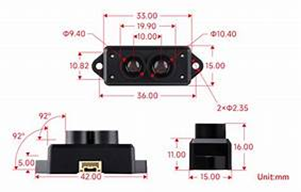
\includegraphics[width=0.8\linewidth]{Carpeta tecnica/Imagen3.png}
    \caption{Proporciones del modulo}
\end{figure}


\subsection{Conversor TTL a USB}

El CP2102 es un controlador de puente USB a UART altamente integrado que permite la conversión directa entre interfaces USB y serie. Este dispositivo es ideal para actualizar sistemas que originalmente utilizaban comunicación RS-232, TTL o RS-485, eliminando la necesidad de puertos seriales tradicionales en PCs modernas.  
Gracias a su tamaño compacto y a la mínima cantidad de componentes externos necesarios, el CP2102 ofrece una solución eficiente, confiable y económica para la comunicación entre ordenadores y dispositivos embebidos.

\begin{figure}[H]
\centering
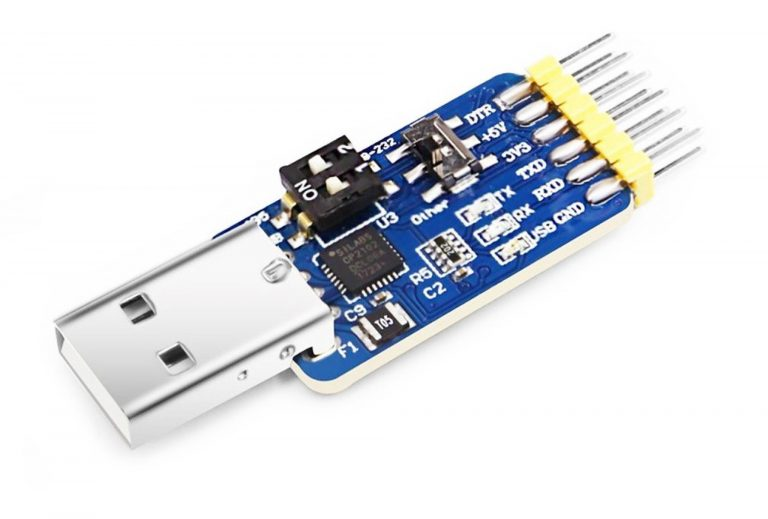
\includegraphics[width=0.6\linewidth]{Carpeta tecnica/Uartransf.png}
\caption{Conversor Serie TTL a USB}
\end{figure}


\subsubsection{Funcionamiento}
El CP2102 actúa como un puente entre la interfaz USB 2.0 y los protocolos UART, RS-232 o RS-485 del dispositivo conectado.  
El chip convierte los datos USB en señales serie y viceversa, facilitando la transmisión y recepción asíncrona de datos.  
El módulo no requiere componentes externos USB y es reconocido automáticamente por la mayoría de los sistemas operativos mediante drivers integrados.

\begin{table}[H]
    \centering
\begin{tabular}{|>{\raggedright}p{5cm}|>{\raggedright\arraybackslash}p{8cm}|}
\hline
\textbf{Parámetro} & \textbf{Valor / Descripción} \\
\hline
Chip principal & CP2102 – Puente USB - UART \\
\hline
Interfaz USB & USB 2.0 (Full Speed, 12 Mbps) \\
\hline
Protocolos soportados & TTL, RS-232, RS-485 \\
\hline
Modos de conversión & USB-TTL, USB-RS232, USB-RS485, TTL-RS232, TTL-RS485, RS232-RS485 \\
\hline
Tamaño & 32 mm × 18 mm \\
\hline
Voltajes soportados & 3.3 V / 5 V \\
\hline
Salidas de potencia & 5 V – 500 mA / 3.3 V – 100 mA \\
\hline
Velocidad máxima & Hasta 2 Mbps \\
\hline
Compatibilidad MCU & 8051, STC, AVR, ARM, STM32, DSP, FPGA, MSP430, etc. \\
\hline
Señales adicionales & DTR, RTS (descarga BSL para MSP430) \\
\hline
Protección & Fusible autorrearmable ante sobrecorriente (>500 mA) \\
\hline
\end{tabular}
\caption{Tabla de características técnicas}
\end{table}

\subsubsection{Funciones Destacadas}
\begin{itemize}
    \item Módulo 6 en 1: Conversión bidireccional entre múltiples interfaces serie.
    \item Compatibilidad con 3.3 V y 5 V: Ideal para microcontroladores modernos de bajo voltaje.
    \item Salidas de alimentación integradas: Posibilidad de alimentar el sistema objetivo durante la depuración.
    \item Protección contra sobrecorriente: Fusible de recuperación automática integrado.
    \item Indicadores LED: Visualización del flujo de datos en transmisión y recepción.
    \item Control automático RS-485: No requiere líneas adicionales de control.
    \item Transferencia libre entre protocolos: Conmutación física confiable sin interferencias.
\end{itemize}

\subsection{Fuente Step-down}
Un buck converter (convertidor reductor) es un convertidor DC-DC que reduce una tensión de entrada (Vin) a un valor menor de salida (Vout), manteniendo una alta eficiencia gracias al uso de conmutación en lugar de disipación resistiva.

En este caso, el regulador está basado en el XL4015, un chip controlador step-down con capacidad de hasta 5 A y frecuencia de trabajo en torno a 180 kHz.

\begin{figure}[H]
\centering
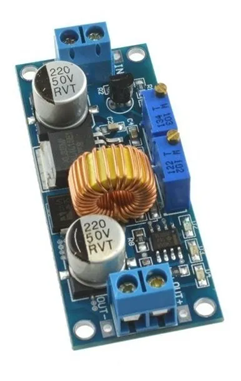
\includegraphics[width=0.5\linewidth]{Carpeta tecnica/Imagen4.png} % Imagen de la fuente step-down
\caption{Fuente buck step-down 5V}
\end{figure}

\subsubsection{Funcionamiento}

El XL4015 regula la salida usando PWM de alta frecuencia y los siguientes componentes externos:

\begin{itemize}

\item MOSFET interno (dentro del XL4015): conmuta la corriente desde la entrada hacia la bobina.

\item Inductor (L1): almacena energía en forma de campo magnético y la entrega suavizada a la carga.

\item Diodo Schottky (D1, SS54): permite el flujo de corriente cuando el MOSFET está apagado, garantizando continuidad de corriente.

\item Capacitores (C1, C2, C3, C4, C5): filtran el rizado de entrada y salida.

\item Resistencias R1 y R2 (red de realimentación): forman un divisor que regula la tensión de salida comparándola con la referencia interna del chip.

\item R3 y C6: compensación y estabilidad del lazo de control.

\item Potenciómetro: ajusta la tensión de salida.

\end{itemize}

\subsubsection{Etapas}

\begin{enumerate}
\item Fase de Conducción (MOSFET ON)

El MOSFET interno del XL4015 se enciende. La corriente fluye desde Vin → L1 → C4/C5 → Carga. La bobina almacena energía en su campo magnético, aumentando su corriente.

\item Fase de Retención (MOSFET OFF)

El MOSFET se apaga. La corriente en el inductor no puede caer abruptamente, por lo que el diodo D1 conduce. La energía almacenada en L1 se transfiere hacia la carga y capacitores de salida.

\item Regulación

El divisor resistivo (R1, R2) mide la tensión de salida. Esta señal se compara con una referencia interna (1,25 V típica). El controlador ajusta el duty cycle del PWM del MOSFET interno para mantener la salida estable.
\end{enumerate}

\subsubsection{Parámetros del Esquema}

\begin{figure}
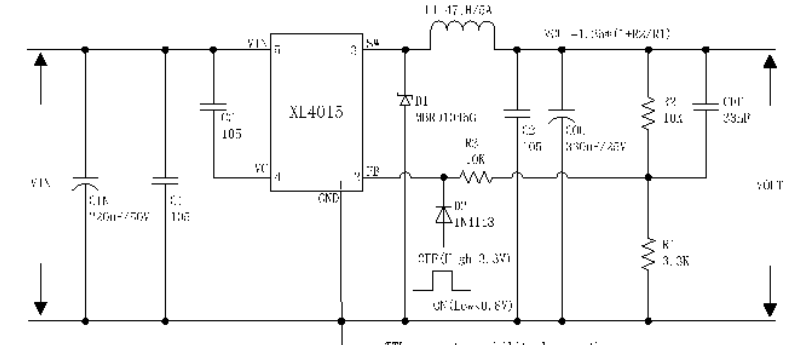
\includegraphics[width=0.9\linewidth]{Carpeta tecnica/esquemastepdown.png}
\caption{Esquemático de Fuente buck step-down}
\end{figure}

\begin{itemize}
\item Chip: XL4015 (regulador step-down DC-DC, hasta 5A).

\item Diodo: SS54 (Schottky, rápido y baja caída de tensión).

\item Inductor: 47 µH, soporta varios amperios.

\item Resistencias: R1 (0,05 $\Omega$ detecta corriente, R2 ajusta Vout.

\item Capacitores:

\begin{itemize}


\item Entrada: 220 µF (electrolítico) + 0,1 µF (cerámico) → filtran ruido y picos de corriente.

\item Salida: 220 µF + 0,1 µF → reducen rizado en Vout.

\end{itemize}
\end{itemize}

\subsection{Baterías}
Las baterías Li-Ion cilíndricas tipo 18650 de 3.7 V y 7800 mAh son acumuladores
recargables de alta capacidad, diseñados para aplicaciones que requieren energía confiable,
autonomía prolongada y recarga eficiente. Su formato estandarizado las hace ampliamente
compatibles con dispositivos electrónicos de consumo y proyectos de ingeniería.
Figura 3.14: Baterías de litio

\begin{figure}[H]
    \centering
    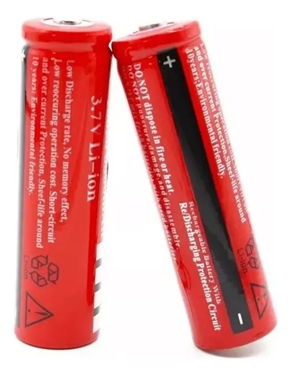
\includegraphics[width=0.5\linewidth]{Carpeta tecnica/Imagen5.png}
    \caption{Baterías recargables}
    \label{fig:placeholder}
\end{figure}

\subsubsection{Características Técnicas}

\begin{itemize}
\item Química: Ion de Litio (Li-ion).

\item Formato: Cilíndrico 18650 (18 mm diámetro × 65 mm longitud).

\item Voltaje nominal: 3,7 V.

\item Voltaje máximo de carga: 4,2 V.

\item Voltaje de corte (descarga): 2,5–3,0 V.

\item Capacidad nominal: 7800 mAh (7,8 Ah).

\item Energía aproximada: ~28,9 Wh por celda.

\item Conectividad: Terminales planos, aptos para soldadura o porta pilas.
\end{itemize}

\subsection{Motores de vibración}
Los motores de vibración que vamos a utilizar son motores de corriente continua (DC) conocidos como Eccentric Rotating Mass (ERM). Su principio de funcionamiento es muy sencillo pero efectivo: El motor tiene un eje que gira cuando se le aplica energía eléctrica. Lo que crea la vibración es un pequeño peso o masa que está unido al eje, pero no en su centro. Este desplazamiento del centro de masa hace que la rotación sea desequilibrada. A medida que el motor gira a alta velocidad, la masa descentrada genera una fuerza centrífuga que cambia de dirección constantemente. Este movimiento rápido y desequilibrado es lo que produce la vibración que se siente. En muchos dispositivos como es el caso de blindassist que requieren retroalimentación háptica, se usan comúnmente dos motores ERM de diferentes tamaños. Esto permite generar distintos niveles de vibración, desde un temblor fuerte y notorio hasta una vibración suave y sutil, mejorando la experiencia del usuario.

\begin{figure}[H]
    \centering
    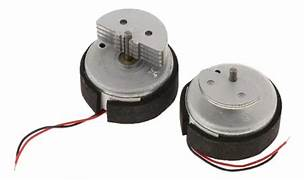
\includegraphics[width=0.5\linewidth]{Carpeta tecnica/Motores.png}
    \caption{Motores de vibración}
\end{figure}

\subsection{Circuito}

\subsubsection{Lista de Componentes}
\begin{longtable}{|>{\raggedright}p{4cm}|c|>{\raggedright\arraybackslash}p{8cm}|}
\hline
\textbf{Componente} & \textbf{Cantidad} & \textbf{Descripción / Función} \\
\hline
Raspberry Pi 4 (J5) & 1 & Microprocesador central, adquisición de datos y control \\
\hline
Sensor TFmini (J1, J2, J3) & 3 & LIDAR para medir distancias \\
\hline
Motores de vibración (J6, J7) & 2 & Generación de señal haptica de alerta \\
\hline
Transistor BC337 (Q1, Q2) & 2 & Etapa de potencia para buzzers \\
\hline
Resistencias 510 $\Omega$ (R1, R2) & 2 & Limitación de corriente en base de transistores \\
\hline
Interruptores (J4, J8) & 2 & Habilitación/deshabilitación manual \\
\hline
Alimentación de baterias (J9, J10) & 2 & Alimentacion de la Raspberry Pi 4 y de los motores de vibración)\\
\hline
\caption{Tabla de la lista de componentes del circuito}
\end{longtable}

%--------------------------
\subsubsection{Descripción del circuito}
\begin{enumerate}
    \item Los sensores TFmini (J1, J2, J3) envían datos de distancia vía UART a la Raspberry Pi 4 (J5).
    \item La Raspberry Pi recibe y procesa la información. Si la distancia medida es menor a un umbral, activa una salida GPIO.
    \item El GPIO activa Q1 o Q2 mediante las resistencias R1 y R2.
    \item Los transistores permiten el paso de corriente hacia los motores (J6, J7), que generan la alerta haptica de vibración.
    \item Los interruptores J4 y J8 permiten habilitar/deshabilitar la deteccion de la IA y seleccionar modos de funcionamiento.
\end{enumerate}

\subsubsection{Esquematico}

\begin{figure}[H]
    \centering
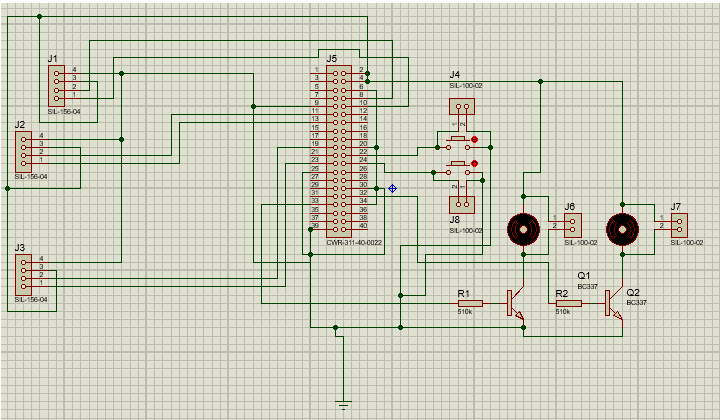
\includegraphics[width=\linewidth]{Carpeta tecnica/Captura de pantalla (1).png}
\caption{Esquematico del circuito final}
\end{figure}


\subsubsection{PCB}

\begin{figure}[H]
    \centering
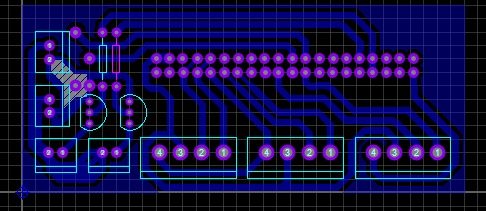
\includegraphics[width=\linewidth]{Carpeta tecnica/nuevo PCB.jpg}
\caption{diseño de impresion del circuito}
\end{figure}

\separador

%--- Firmware ---
\section{Firmware}

\subsection{Detección por IA}
El sistema de visión artificial implementado en este proyecto se basa en el modelo de aprendizaje profundo YOLOv8n.pt para la identificación de objetos en tiempo real, utilizando la cámara de la Raspberry Pi como fuente de datos. La arquitectura del software se estructura en un sistema de Programación Orientada a Objetos (POO). Cada componente lógico (cámara, IA, voz, traductor) está encapsulado en una clase dedicada, lo que facilita el desarrollo, las pruebas y el mantenimiento del sistema de manera modular.

\begin{figure}[H]
\noindent\hspace*{-0.7in}% desplaza hacia la izquierda el origen
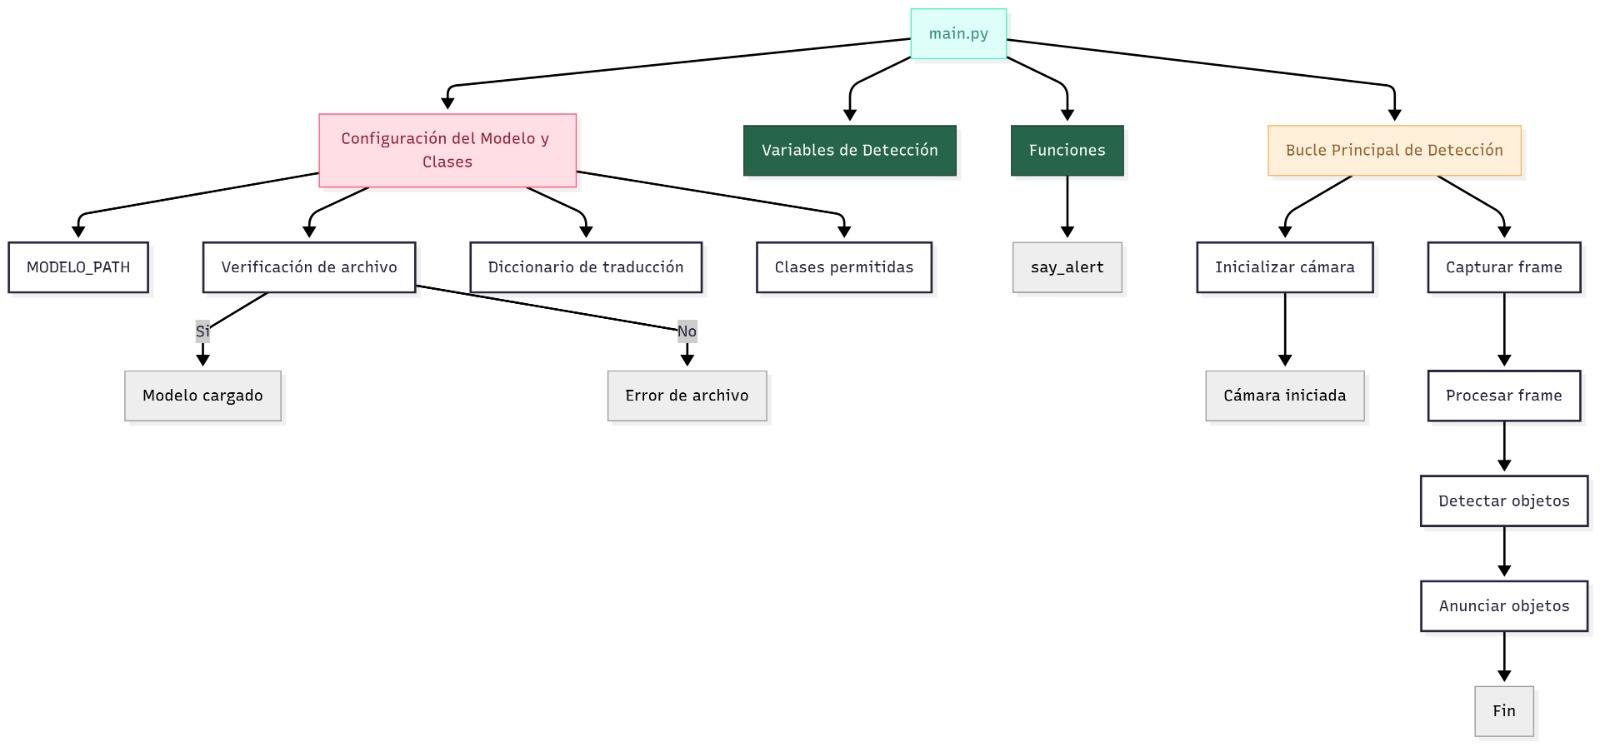
\includegraphics[width=1.2\linewidth]{Carpeta tecnica/diagramaflujoia1.jpg}
\caption{Diagrama de flujo de la deteccion por IA}
\end{figure}

\subsubsection{logica del bucle continuo}
\begin{itemize}
\item Captura frames de video.
\item Analiza cada frame en busca de objetos.
\item Compara las detecciones con las del frame anterior.
\item Emite una alerta de voz solo cuando se detecta un cambio en el entorno (aparición o desaparición de un objeto).
\end{itemize}

\subsubsection{Arquitectura del Código}
El programa se organiza en un conjunto de clases principales:
\begin{itemize}
\item \textbf{Clase Camara:} Gestiona el hardware de la cámara. Utiliza la librería picamera2 para inicializar y capturar un stream de video en vivo. A diferencia de soluciones de un solo fotograma, esta aproximación optimiza el rendimiento y la tasa de fotogramas por segundo (FPS) al mantener el stream de video abierto.
\item \textbf{Clase IA:} Actúa como el motor de inteligencia artificial. Carga el modelo yolov8n.pt y es responsable de analizar los fotogramas capturados. Identifica objetos en una lista predefinida de clases (clases\_permitidas) y filtra las detecciones por un umbral de confianza (CONFIDENCE\_THRESHOLD), asegurando que solo los objetos relevantes y con alta certeza sean considerados.
\item \textbf{Clase Traductor:} Encapsula el diccionario de traducciones. Su única responsabilidad es convertir los nombres de las clases de YOLO (en inglés, como 'person' o 'car') a sus equivalentes en español, permitiendo que el sistema de voz dé las alertas en el idioma del usuario.
\item \textbf{Clase Voz:} Maneja la síntesis de voz. Para garantizar la fiabilidad del audio, utiliza un método robusto basado en la librería subprocess para ejecutar el comando del sistema espeak y vocalizar las alertas. Esta solución es inmune a los problemas de configuración de audio que se presentan a menudo con otras librerías.
\item \textbf{Clase Main:} Es el orquestador principal del sistema. Inicializa todas las demás clases y gestiona el bucle de detección en tiempo real. Su lógica más avanzada reside en el método privado \_\_anunciar\_detecciones, que compara las detecciones actuales con las del último ciclo, emitiendo una alerta de voz únicamente cuando se detecta un cambio. Esto evita la repetición constante de las mismas alertas.
\end{itemize}
El sistema se ejecuta continuamente en un bucle while hasta que el usuario lo interrumpe con Ctrl + C. En ese momento, un bloque finally asegura que el hardware de la cámara se detenga de manera segura para evitar fallos del sistema.

\begin{figure}[H]
\noindent\hspace*{-0.7in}% desplaza hacia la izquierda el origen
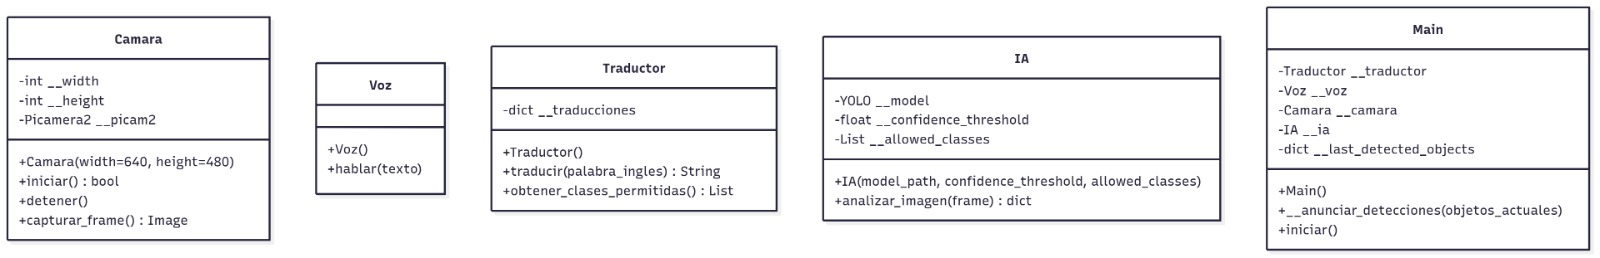
\includegraphics[width=1.2\linewidth]{Carpeta tecnica/Diagramaflujoia2.jpg}
\caption{Diagrama de flujo de clases}
\end{figure}

\subsubsection{Componentes de la Implementación}
\paragraph{Librerías}
\begin{itemize}
\item ultralytics: Se utiliza para cargar y ejecutar el modelo de detección de objetos YOLOv8.
\item picamera2: La interfaz oficial para las cámaras de la Raspberry Pi, proporcionando acceso a un flujo de video de alto rendimiento.
\item cv2 (OpenCV): Se usa para el preprocesamiento de los fotogramas, como la conversión de color necesaria antes de pasarlos al modelo de IA.
\item subprocess: La herramienta estándar de Python para ejecutar comandos del sistema, en este caso, el motor de síntesis de voz espeak.
\item os y sys: Permiten la gestión de archivos y el control del sistema, por ejemplo, para verificar la existencia del modelo YOLO antes de su uso.
\end{itemize}

\paragraph{Manejo de Flujo de Datos}
El flujo de información y la lógica de control se manejan principalmente en el método iniciar() de la clase Main:
\begin{itemize}
\item \textbf{Captura:} self.\_\_camara.capturar\_frame() obtiene una imagen del stream de la cámara.
\item \textbf{Análisis:} El frame se pasa a self.\_\_ia.analizar\_imagen(frame), que devuelve un diccionario con los objetos detectados en el fotograma actual.
\item \textbf{Control de Anuncios:} El diccionario se envía al método \_\_anunciar\_detecciones().
\item \textbf{Reproducción de Audio:} Si hay cambios, la clase Voz es invocada a través de self.\_\_voz.hablar(final\_message).
\end{itemize}
La arquitectura del sistema es muy escalable. Al estar modularizado, se podrían añadir fácilmente nuevas clases sin modificar la lógica central del proyecto.

\subsection{Detección por láser}
\subsubsection{Libreria TFmini}
Esta sección describe el funcionamiento del código implementado para la lectura simultánea de tres sensores LiDAR TFmini conectados a diferentes puertos UART de una Raspberry Pi 4.

El sistema permite:
\begin{itemize}
\item Recepción continua de datos desde los sensores.
\item Procesamiento y almacenamiento de las distancias medidas.
\item Ejecución en paralelo mediante hilos (multithreading).
\item Disponibilidad centralizada de los valores para otras funciones del sistema.
\end{itemize}

\textbf{Descripción General del Sistema:}
El programa se estructura en cuatro bloques principales:
\begin{itemize}
\item Configuración global: Definición de librerías, estructuras de datos y variables compartidas.
\item Módulo de adquisición de datos: Funciones de lectura desde los sensores a través de los puertos UART.
\item Gestión de hilos: Creación de procesos concurrentes para la lectura simultánea.
\item Bucle principal: Supervisión e impresión periódica de los valores capturados.
\end{itemize}
La arquitectura se basa en la comunicación serial estándar (UART) a una velocidad de 115200 baudios, con tramas de 9 bytes emitidas por cada TFmini.

\paragraph{Librerías:}
\begin{itemize}
\item \textbf{serial (pyserial):} Permite abrir, configurar y gestionar la comunicación UART.
\item \textbf{time:} Se utiliza para pausas entre lecturas y evitar sobrecarga del procesador.
\item \textbf{threading:} Facilita la ejecución concurrente de múltiples lecturas de sensores.
\end{itemize}

\paragraph{Estructuras Globales:}
\begin{verbatim}
distancias = {
"uart1": None,
"uart2": None,
"uart3": None,
}
\end{verbatim}
Diccionario que almacena la última distancia válida obtenida de cada sensor. Inicialmente los valores son None y se actualizan en tiempo real. Facilita la consulta de datos desde cualquier parte del programa.

\paragraph{Función Genérica de Adquisición de Datos:}

\begin{verbatim}
def getTFminiData(port, key_name):
ser = serial.Serial(port, 115200, timeout=1)
\end{verbatim}

\textbf{Flujo de la función:} 
Apertura del puerto serie con parámetros: Velocidad de 115200 baudios, timeout de 1 segundo. Bucle infinito de lectura: Verifica si hay al menos 9 bytes disponibles (ser.in\_waiting > 8). Lee un paquete completo (ser.read(9)). Validación de cabecera: Primeros dos bytes deben ser 0x59 0x59. Si no coincide, se descarta la trama. Reconstrucción de la distancia: Byte [2] = parte baja (Low). Byte [3] = parte alta (High). Cálculo: distance = low + (high << 8).

\end{quoting}

\paragraph{Almacenamiento de datos}
La distancia calculada se guarda en el diccionario global bajo la clave correspondiente (uart1, uart2, uart3). Retardo de control time.sleep(0.01) para liberar recursos del procesador.

\paragraph{Funciones Específicas por Puerto UART}

\begin{verbatim}
def getTFminiData_uart1():
getTFminiData("/dev/serial0", "uart1")
\end{verbatim}
Función getTFminiData\_uart1: Llama al puerto /dev/serial0. Función getTFminiData\_uart2: Llama al puerto /dev/ttyUSB1. Función getTFminiData\_uart3: Llama al puerto /dev/ttyUSB2. Estas funciones permiten escalar el sistema sin modificar la lógica principal.

\paragraph{Gestión de Hilos y Ejecución Principal}
\begin{verbatim}
if __name__ == '__main__':
...
\end{verbatim}
Creación de hilos: Cada hilo ejecuta una de las funciones específicas (uart1, uart2, uart3). Se utilizan hilos daemon, lo que asegura que se cierren cuando termine el programa. Ejecución concurrente: Los tres hilos inician en paralelo con .start(). Se garantiza la lectura simultánea de los sensores. Bucle principal de supervisión: Cada segundo imprime las distancias almacenadas en distancias y permite monitorear en consola el funcionamiento del sistema. Interrupción del usuario: Al presionar Ctrl + C, se captura la excepción KeyboardInterrupt. Se muestra un mensaje de salida segura.

\begin{figure}[H]
\noindent\hspace*{-0.7in}% desplaza hacia la izquierda el origen
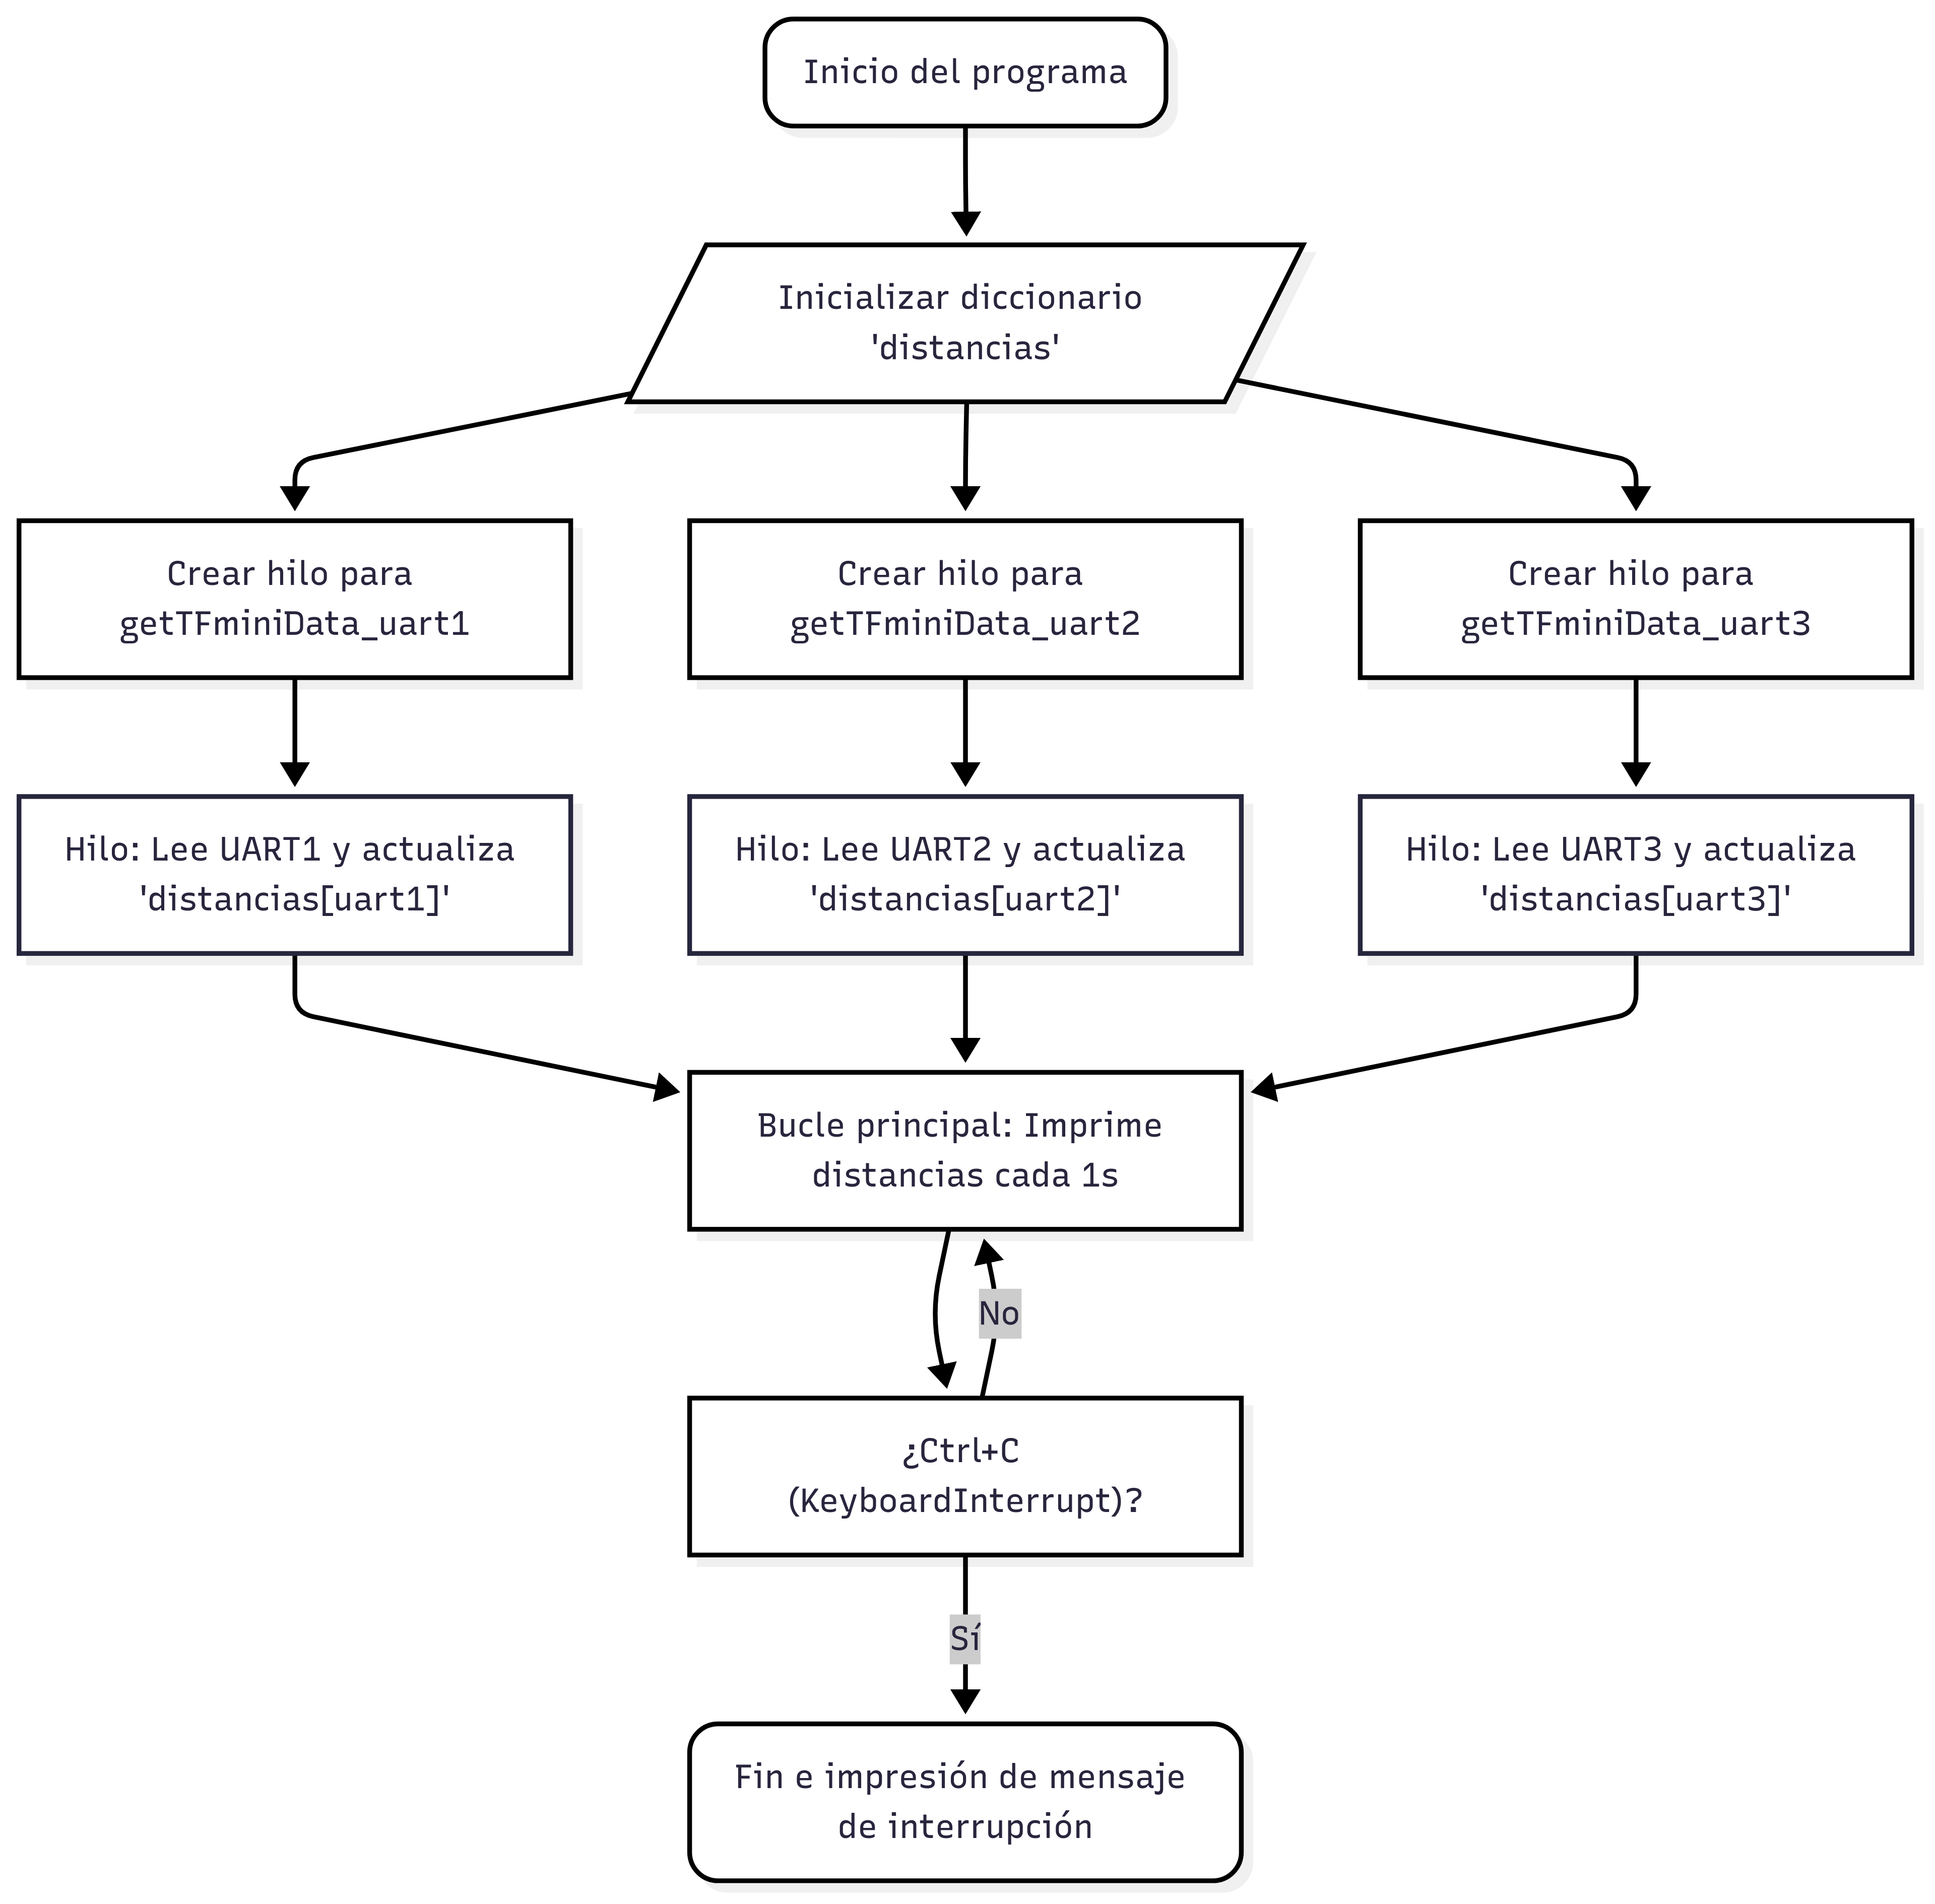
\includegraphics[width=1.2\linewidth,height=1.1\linewidth]{Carpeta tecnica/diagrama de flujo TFmini3.png}
\caption{Diagrama de flujo de la lectura de distancias}
\end{figure}

\subsubsection{Control de Motores}

El código implementa un sistema de control de dos motores mediante modulación por ancho de pulso (PWM) utilizando una Raspberry Pi 4.  
El control se basa en las distancias medidas por tres sensores LiDAR TFmini conectados a los puertos UART de la Raspberry Pi.  
El objetivo del programa es variar la velocidad de los motores en función de la proximidad de obstáculos, generando alertas hapticas (mediante vibraciones) cuando se detectan objetos a menos de 120 cm.


\paragraph{Librerías y Dependencias}

\begin{itemize}
    \item \texttt{time}: Control de tiempos y retardos.
    \item \texttt{threading}: Permite ejecutar lecturas de los tres sensores en paralelo mediante hilos.
    \item \texttt{RPi.GPIO}: Control de los pines GPIO de la Raspberry Pi.
    \item \texttt{TFtest3}: Módulo externo que contiene las funciones de lectura \texttt{getTFminiData\_uart1/2/3} y el diccionario \texttt{distancias}.
\end{itemize}

\paragraph{Configuración del Sistema}

\begin{itemize}
    \item\textbf{Modo GPIO:}

\begin{verbatim}
GPIO.setmode(GPIO.BCM)
\end{verbatim}

\item\textbf{Asignación de Pines PWM:}
\begin{verbatim}
MOTOR_PIN1 = 18
MOTOR_PIN2 = 13
\end{verbatim}

Estos pines son compatibles con PWM por hardware en la Raspberry Pi 4.

\item\textbf{Inicialización de PWM:}
\begin{verbatim}
pwm1 = GPIO.PWM(MOTOR_PIN1, 100)
pwm2 = GPIO.PWM(MOTOR_PIN2, 100)
pwm1.start(0)
pwm2.start(0)
\end{verbatim}

Se inicializan ambas salidas con una frecuencia de \textbf{100 Hz} y un duty cicle del \textbf{0 \%}.
\end{itemize}

\paragraph{Función Auxiliar}
\begin{itemize}
\texttt{calcular\_duty(d):} Esta función traduce la distancia medida (en cm) al porcentaje de ciclo útil del PWM.  
Si el objeto está a menos de \textbf{120 cm}, el duty cycle aumenta proporcionalmente al acercamiento.

\begin{verbatim}
if d < 120:
    return min(100, 120 - d)
\end{verbatim}

Ejemplo de funcionamiento:
\begin{itemize}
    \item Si $d = 100$ cm $\rightarrow$ $duty = 20\%$
    \item Si $d = 50$ cm $\rightarrow$ $duty = 70\%$
\end{itemize}
\end{itemize}

\paragraph{Lógica de Control Principal}
\begin{itemize}

Función central que coordina la lectura de los tres sensores y actualiza los dos motores según las condiciones detectadas.

\textbf{Ciclo de operación:}

\begin{enumerate}
    \item Reinicia el PWM en 0\% al comienzo de cada ciclo.  
    \item Lee las distancias \texttt{d1}(Sensor derecho), \texttt{d2}(Sensor izquierdo), \texttt{d3}(Sensor frontal) desde el diccionario compartido \texttt{distancias}.  
    \item Calcula los valores de duty correspondientes.  
    \item Evalúa las condiciones de proximidad menores a 120 cm.  
\end{enumerate}

\textbf{Casos contemplados:}

\begin{table}[H]
\centering
\begin{tabular}{|c|p{5cm}|p{7cm}|}
\hline
\textbf{Caso} & \textbf{Condición} & \textbf{Acción} \\ \hline
1 & d1 $<$ 120 & Activa PWM0 proporcionalmente. \\ \hline
2 & d2 $<$ 120 & Activa PWM1 proporcionalmente. \\ \hline
3 & d3 $<$ 120 & Ambos motores actúan con el mismo PWM. \\ \hline
4 & d2 y d3 $<$ 120 & Motor 2 titila alternadamente. \\ \hline
5 & d1 y d3 $<$ 120 & Motor 1 titila alternadamente. \\ \hline
6 & d1, d2 y d3 $<$ 120 & Ambos motores al 100\% (alerta crítica). \\ \hline
\end{tabular}
\caption{Casos de control de motores según distancias detectadas.}
\end{table}
\end{itemize}

\paragraph{Ejecución Principal}

\begin{itemize}
El bloque \texttt{if \_\_name\_\_ == "\_\_main\_\_":} inicia la ejecución del programa.

Se crean tres hilos dedicados a la lectura continua de los sensores TFmini:

\begin{verbatim}
t1 = threading.Thread(target=getTFminiData_uart1, daemon=True)
\end{verbatim}

Un cuarto hilo ejecuta la función \texttt{control\_sensores()} para el control de los motores.  
El bucle principal mantiene el programa activo indefinidamente mientras los hilos trabajan en segundo plano.
\end{itemize}

\paragraph{Finalización Segura}
\begin{itemize}
En caso de interrupción manual (Ctrl + C), el programa detiene los PWM y limpia la configuración de los GPIO:

\begin{verbatim}
pwm1.stop()
pwm2.stop()
GPIO.cleanup()
\end{verbatim}

Esto evita errores en ejecuciones posteriores.
\end{itemize}

\begin{figure}[H]
    \centering
    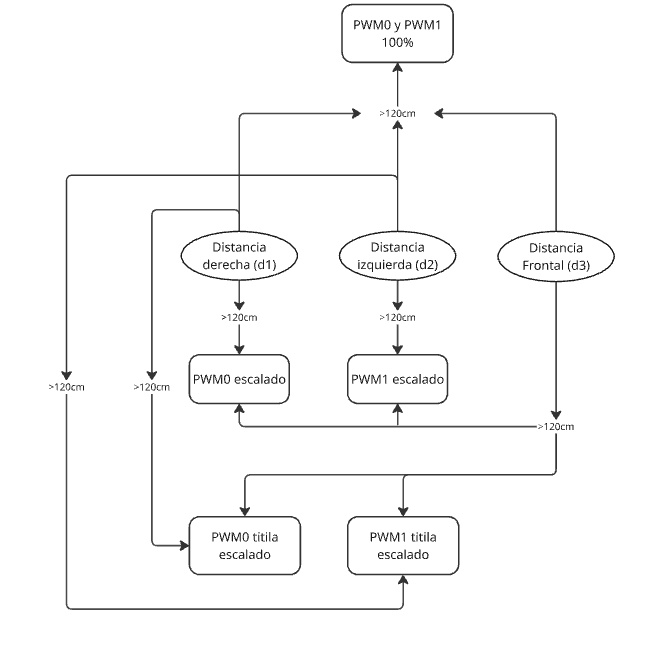
\includegraphics[width=\linewidth]{Carpeta tecnica/diagrama PWM.png}
    \caption{Diagrama de flujo e la logica PWM}
\end{figure}

\subsubsection{Código Final del Control Principal (control\_principal.py)}

La función principal de este script es coordinar todos los módulos de hardware y software: cámara, sensores LiDAR, motores de vibración y el sistema de voz. Gracias a esta integración, el dispositivo puede ofrecer detección de objetos y advertencia de obstáculos de manera simultánea y en tiempo real.

\paragraph{Importación de Librerías y Configuración}

\begin{itemize}
Al inicio, el código importa distintas librerías necesarias para manejar el hardware y los módulos de inteligencia artificial:
\end{itemize}


\begin{verbatim}
import RPi.GPIO as GPIO
import threading
import time
import cv2
from ultralytics import YOLO
\end{verbatim}

En términos generales, estas librerías permiten conectar la Raspberry Pi con el entorno físico (botones, motores, cámara), al mismo tiempo que se integra el modelo de IA encargado de reconocer objetos.

\paragraph{Gestión de Pines y Estados Globales}
\begin{itemize}

El sistema trabaja con botones y motores conectados a pines GPIO de la Raspberry Pi. Estos pines permiten encender o apagar funciones al pulsar un botón y regular la intensidad de vibración de los motores mediante señales PWM.

\end{itemize}

\begin{verbatim}
PIN_DETECCION = 25   # Botón para activar la cámara
PIN_LIDAR = 8        # Botón para activar el LiDAR
MOTOR_PIN1 = 18
MOTOR_PIN2 = 13
\end{verbatim}

De este modo, el usuario puede elegir si activa la detección de objetos o el aviso de obstáculos, cada uno ejecutado en hilos separados.

\paragraph{Lógica Multihilo (Threads)}
  
\begin{itemize}
El programa aprovecha la librería threading para ejecutar varias tareas al mismo tiempo.
    \item Al presionar el botón de detección, se inicia un hilo que activa la cámara y el modelo de IA. Este módulo captura imágenes, analiza lo que ve y notifica mediante voz qué objetos han aparecido o desaparecido en el entorno.
    \item Al presionar el botón de LiDAR, se inician varios hilos que leen la distancia desde los sensores y controlan los motores de vibración. Cuanto más cerca esté un obstáculo, más intensa es la vibración.
\end{itemize}

De esta forma, el usuario recibe información visual traducida tanto en mensajes de voz como en señales hápticas.

\paragraph{Manejo de Eventos con GPIO}
\begin{itemize}
El sistema está preparado para reaccionar automáticamente cuando se presiona un botón. Esto se logra configurando los pines de entrada de la Raspberry Pi con interrupciones:
\end{itemize}

\begin{verbatim}
GPIO.add_event_detect(PIN_DETECCION, GPIO.FALLING, 
                      callback=boton_callback, bouncetime=300)
\end{verbatim}

La función \texttt{boton\_callback()} determina qué botón fue presionado y activa o desactiva el hilo correspondiente. Si un módulo ya estaba en ejecución, el mismo botón permite detenerlo.

\paragraph{Función Principal (main)}


El núcleo del programa es la función \texttt{main()}, que inicia el sistema, espera unos segundos para asegurar que todo el hardware esté listo, y finalmente queda a la espera de que el usuario presione algún botón:

\begin{verbatim}
def main():
    print("[INFO] Esperando 10 segundos...")
    time.sleep(10)
    iniciar_gpio()
    voz = Voz()
    voz.hablar("Sistema listo para operar.")
\end{verbatim}

Esto asegura un arranque limpio y confiable.

\paragraph{Procedimiento de Despliegue y Arranque Automático}

\begin{itemize}
Un aspecto fundamental del proyecto fue garantizar que el sistema se ejecute de forma automática al encender la Raspberry Pi. Para ello, se descartó el uso de \texttt{crontab}, que presentaba fallos al iniciar el entorno virtual de Python, y se optó por \texttt{systemd}, la herramienta moderna de Linux para gestionar servicios.
\end{itemize}

\paragraph{Archivo de Servicio: blindassist.service}

\begin{itemize}
El archivo \texttt{blindassist.service}, ubicado en \texttt{/etc/systemd/system/}, define cómo y cuándo debe ejecutarse el programa principal. Su contenido clave es:
\end{itemize}

\begin{verbatim}
[Unit]
Description=Servicio de Asistencia Visual - Arranque Automatico
After=network.target multi-user.target

[Service]
Type=idle
User=blindassist
ExecStart=/bin/bash -c "sleep 10 && 
/home/blindassist/repo/firmware/.venv/bin/python 
/home/blindassist/repo/firmware/control_principal.py"
Restart=always
RestartSec=5

[Install]
WantedBy=multi-user.target
\end{verbatim}

Este archivo cumple con tres funciones principales:
\begin{itemize}
    \item \textbf{Arranque Diferido:} El comando \texttt{sleep 10} garantiza que el sistema operativo haya terminado de cargar antes de iniciar el script.
    \item \textbf{Ejecución en Segundo Plano:} El programa se ejecuta como un servicio del sistema, independiente de sesiones de usuario.
    \item \textbf{Robustez:} En caso de fallo, el servicio se reinicia automáticamente gracias a las directivas \texttt{Restart=always} y \texttt{RestartSec=5}.
\end{itemize}

\separador

%--- Diseño ---
\section{Diseño}

\subsection*{ Prototipo 3D}

\subsection*{ Materiales Utilizados / Programas}
\begin{itemize}
\item Filamento de impresión 3D PLA.
\item Tornillos 1/8
\item AutoCAD
\end{itemize}

\subsection{Diseño General}
El diseño corresponde a un prototipo de carcasa destinado a integrar de forma eficiente los sensores y componentes del proyecto. Su geometría incluye un frente inclinado en forma triangular, que permite optimizar los ángulos de medición de los LIDAR y ampliar su campo de detección en entornos urbanos. También incorpora un orificio frontal para la cámara y tres ranuras específicas para los LIDAR, lo que asegura una orientación precisa y funcional. El sistema de cierre se resuelve mediante anclajes en el borde del cuerpo y orejas externas para tornillos, lo que garantiza un ajuste firme y facilita el mantenimiento. A nivel general, el prototipo busca maximizar el aprovechamiento del espacio interno, mejorar la disposición de los sensores y proteger los componentes electrónicos. Es importante remarcar que se trata de un prototipo en evolución, sujeto a mejoras tanto en la disposición interna como en la ergonomía y robustez del ensamble.

\subsection{Comparaciones entre Versiones}
\begin{itemize}
\item \textbf{Espacio interno:} El primer prototipo no contaba con el espacio suficiente para albergar todos los componentes electrónicos. En el segundo, se corrigieron dimensiones y proporciones, logrando una organización más adecuada del volumen interno.
\item \textbf{Ranuras para sensores LIDAR:} En el primer modelo, las ranuras eran más genéricas y no contemplaban bien la orientación de los sensores. El segundo prototipo introdujo tres ranuras específicas para los LIDAR, con un frente inclinado que mejora el ángulo de detección.
\item \textbf{Relieves y fijaciones internas:} El primer y segundo prototipo carecían de soporte interno para los componentes. En el tercer prototipo, que exteriormente mantiene la misma geometría, se añadieron relieves interiores para que los LIDAR queden bien posicionados y se incorporaron finalmente los anclajes para fijar las plaquetas electrónicas, permitiendo un montaje más firme y seguro.
\item \textbf{Sistema de cierre}: Desde el segundo prototipo ya se contemplaban orejas externas para tornillería, pero en el prototipos siguiente se mejoró la definición de los encastres en el borde del cuerpo, logrando un cierre más sólido.
\item La serie de prototipos muestra una mejora constante en la funcionalidad y organización interna de la carcasa. El primer prototipo permitió validar dimensiones generales. El segundo resolvió la correcta orientación de los LIDAR con el frente inclinado y el aumento de espacio. El tercero introdujo finalmente los relieves interiores y fijaciones internas, mejorando la integración de los componentes. Este proceso iterativo confirma que el diseño está en el camino correcto, pero aún con margen para seguir perfeccionando aspectos de robustez estructural, ensamblaje y usabilidad.
\end{itemize}

\subsection{Imágenes}
\subsubsection{Primer Prototipo}
\begin{figure}[H]
    \centering
    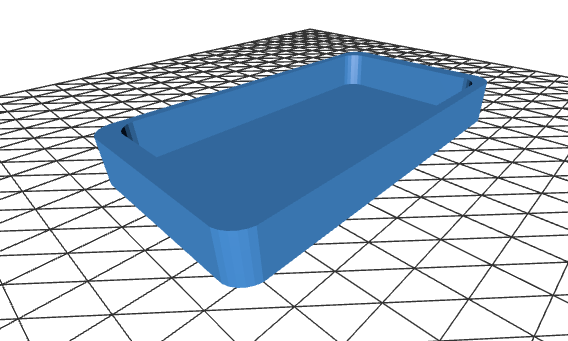
\includegraphics[width=0.5\linewidth]{Carpeta tecnica/modelo baj1.png}
\end{figure}
\begin{figure}[H]
    \centering
    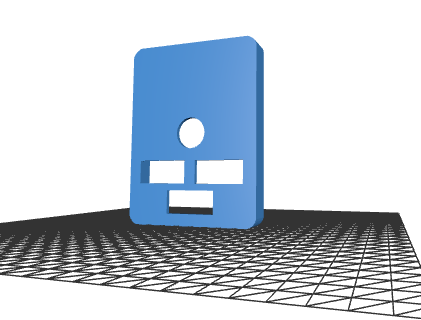
\includegraphics[width=0.5\linewidth]{Carpeta tecnica/primer tapa.png}
    \caption{Primera tapa}
\end{figure}

\subsubsection{Segundo Prototipo}

\begin{figure}[H]
    \centering
    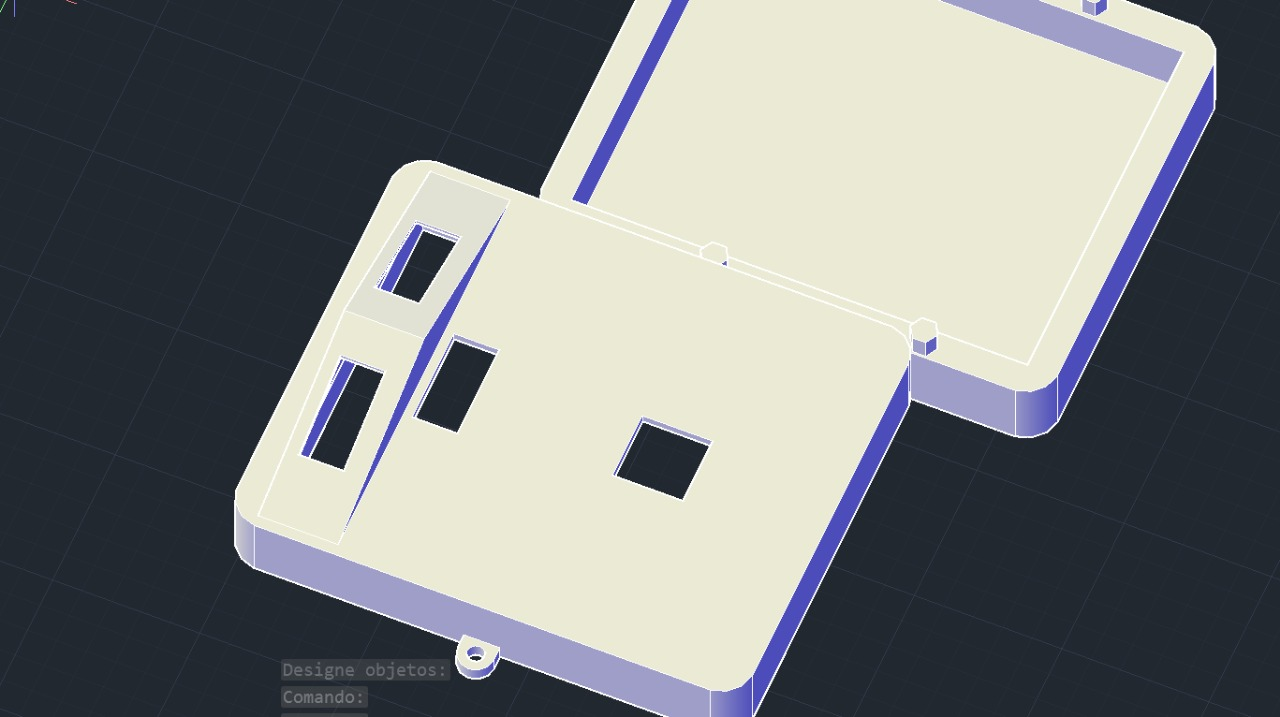
\includegraphics[width=0.5\linewidth]{Carpeta tecnica/segundo proto.png}
    \caption{Tapa y base}
\end{figure}
\separador

%--- Redes sociales ---
\section{Redes sociales}

\subsection{Página web}

\subsection{Lenguajes utilizados. }
\begin{itemize}
\item El proyecto utiliza tres lenguajes principales: HTML, CSS y JavaScript. HTML define la estructura de la página, es decir, organiza el contenido en secciones, títulos, párrafos e imágenes. CSS se encarga de la parte visual, dándole color, tipografía, tamaños, efectos y adaptando el diseño a distintos dispositivos. Por último, JavaScript agrega la interactividad, como las animaciones, el carrusel de imágenes, los gráficos y la lectura en voz alta. En conjunto, HTML estructura, CSS diseña y JavaScript da dinamismo.
\end{itemize}

\subsection{Desglose de Infraestructura}
\subsubsection*{Header/Encabezado}
\begin{itemize}
\item Contenidos: Logo del proyecto, Nombre del proyecto, Slogan, Botón de lectura de contenidos por el narrador, Barra de navegación con todas las secciones de la web.
\item Objetivo: Navegación cómoda, intuitiva y accesibilidad para el grupo objetivo.
\end{itemize}

    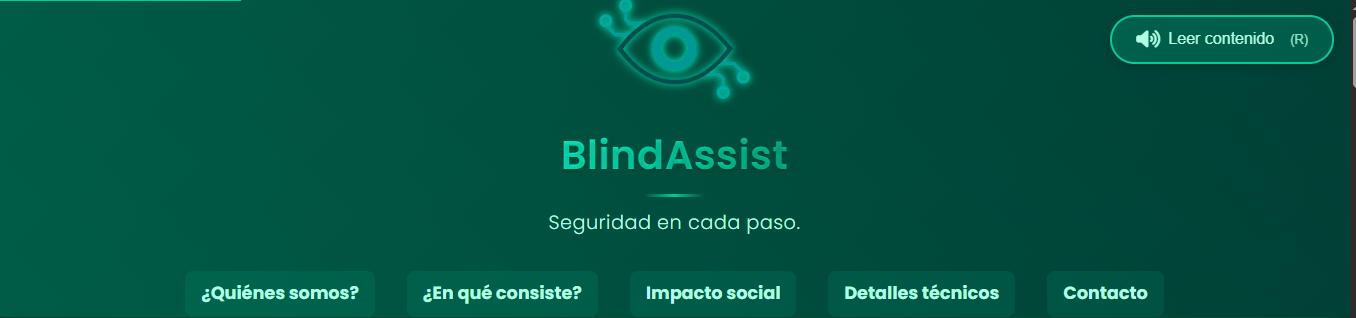
\includegraphics[width=\linewidth]{Carpeta tecnica/header.png}

\subsubsection*{ Sección: ¿Quienes Somos? }
\begin{itemize}
    \item Contenidos: Perfiles de los integrantes del proyecto en recuadros por separado.
    \item Objetivos: Presentación.
\end{itemize}
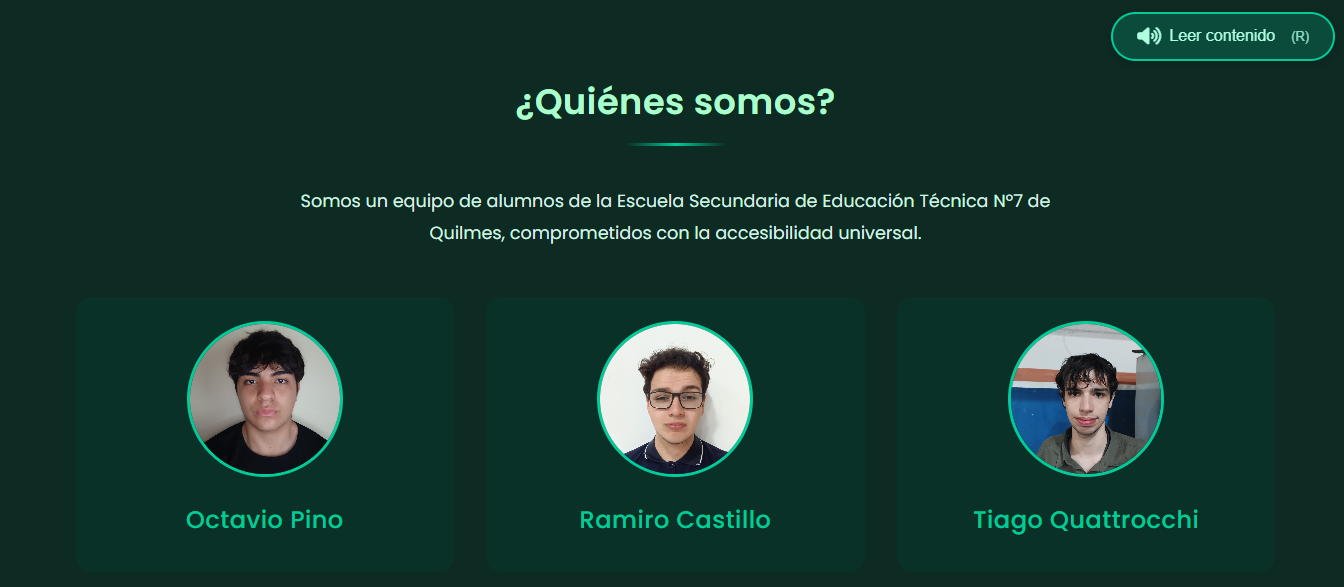
\includegraphics[width=\linewidth]{Carpeta tecnica/qnes.png}
\subsubsection*{ Sección: ¿En qué consiste?}
\begin{itemize}
    \item Contenidos: Texto.
    \item Objetivos: Explicar de manera muy breve el propósito del proyecto.
\end{itemize} 

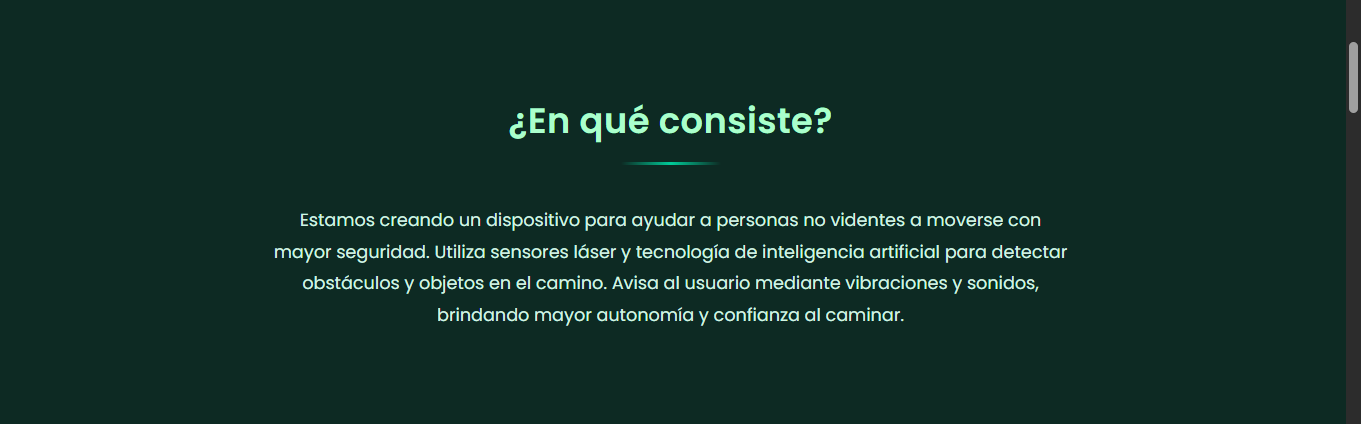
\includegraphics[width=\linewidth]{Carpeta tecnica/cnste.png}

\subsubsection*{Sección: Impacto Social}
\begin{itemize}
    \item Contenidos: Gráficos: Población Ciega Mundial, Distribución por Continente, Distribución por Edad
    \item Objetivos: Concienciar sobre las estadísticas.
\end{itemize}

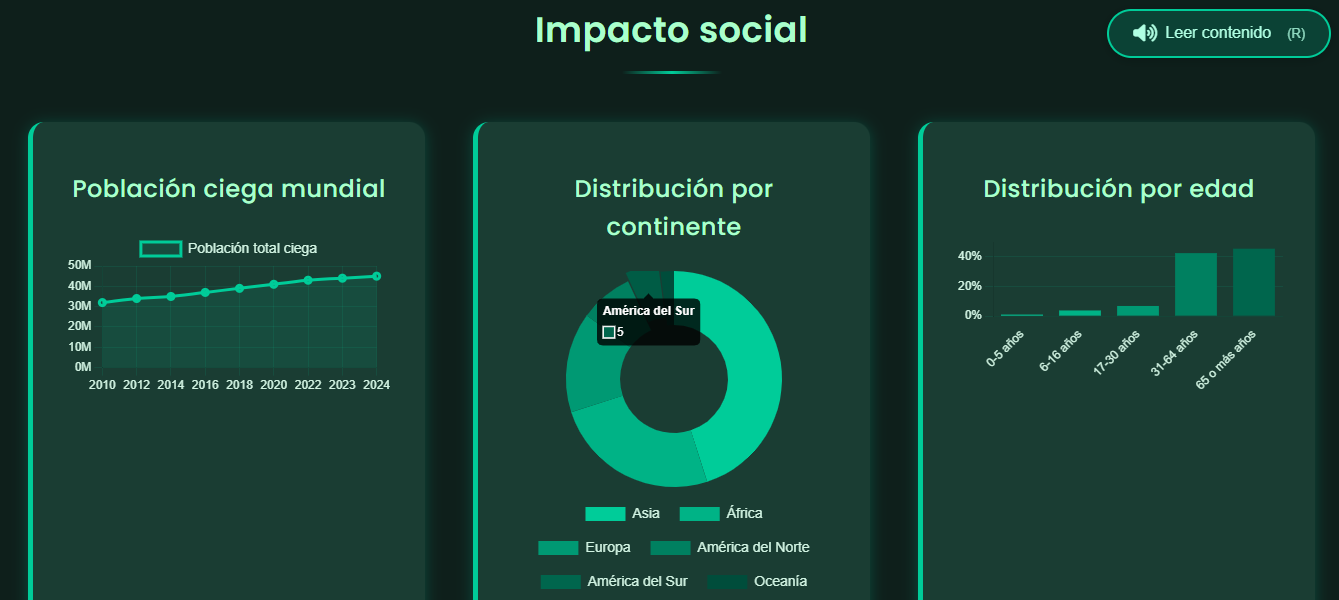
\includegraphics[width=\linewidth]{Carpeta tecnica/grfcs.png}

\subsubsection*{ Sección: Detalles Técnicos}
\begin{itemize}
    \item Contenido: Cuadro de Texto.
    \item Objetivo: Breve explicación enfocada en el funcionamiento de los componentes. 
\end{itemize}

\subsubsection*{Sección: Contacto }
\begin{itemize}
    \item Contenidos: Cuadro de contactos, Link a Instagram.
    \item Objetivo: Comunicarse con nostros.
\end{itemize}

    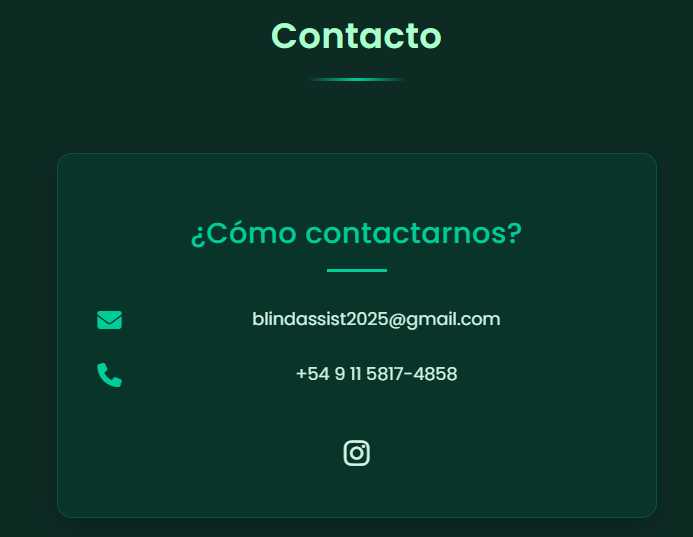
\includegraphics[width=0.5\linewidth]{Carpeta tecnica/cntacto.png}


\subsubsection*{Sección: Galería}
\begin{itemize}
    \item Contenido: Imágenes de presentaciones, proceso, etc.
\end{itemize}


    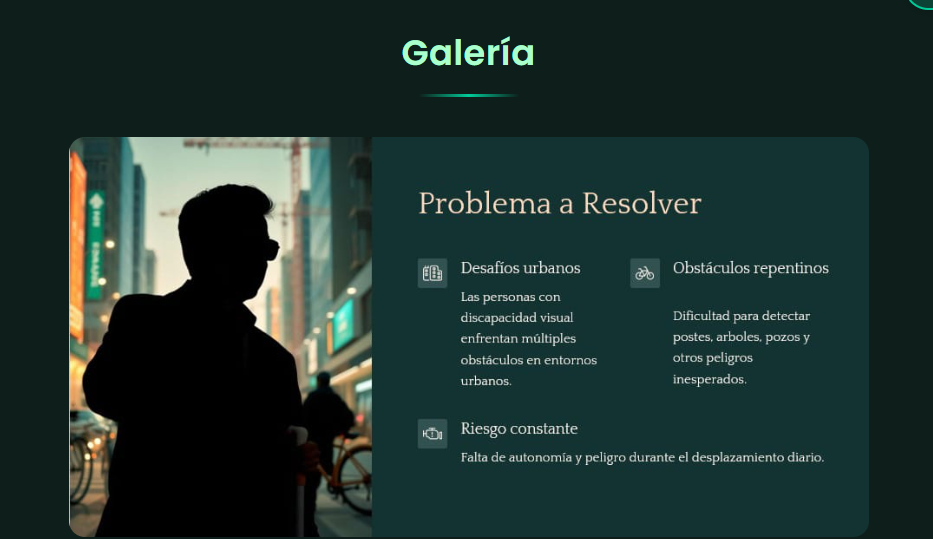
\includegraphics[width=0.5\linewidth]{Carpeta tecnica/galeria.png}


\subsection{Instagram}

\subsubsection{Introducción}
El proyecto BlindAssist cuenta con un perfil en la red social Instagram (@blindassist), utilizado como canal principal de difusión y visibilización. La estrategia digital busca transmitir de manera clara y atractiva los valores del proyecto: innovación, accesibilidad y seguridad.

%--------------------------

\subsubsection{Colores Corporativos}
Se emplea una paleta tecnológica y moderna compuesta por los tonos:
\begin{itemize}
    \item \textcolor{verdeagua}{\#1B9E96}
    \item \textcolor{verdeoscuro}{\#002C2D}
    \item \textcolor{verdemedio}{\#004F4E}
\end{itemize}
Estos colores transmiten confianza, innovación y un enfoque en la accesibilidad.

\subsubsection{Logotipo}
El isotipo está conformado por un ojo integrado con circuitos electrónicos, representando la unión entre la visión y la tecnología.  
El logotipo incluye el nombre BLINDASSIST en una tipografía moderna y clara, pensada para garantizar legibilidad.

\subsubsection{Coherencia Gráfica}
La identidad visual mantiene unidad en todas las piezas gráficas, incluyendo presentaciones, banners y publicaciones digitales, reforzando el reconocimiento de marca.

%---------------------------
\subsubsection{Formato y Planificación de Publicaciones}
\begin{itemize}
    \item El feed combina publicaciones gráficas y material en video corto (\textit{reels}).
    \item Se utilizan banners con información incorporada en algunas imágenes para dar contexto y aportar valor visual a la grilla.
    \item El contenido está planificado de forma ordenada, priorizando la claridad estética y el atractivo visual.
\end{itemize}

%---------------------------
\subsubsection{Reels Publicados}
\begin{itemize}
    \item \textbf{Presentación del sponsor:} se destaca el apoyo recibido para la continuidad del proyecto.
    \item \textbf{Introducción general al proyecto:} explica el objetivo y la propuesta de BlindAssist.
    \item \textbf{Recepción de componentes:} muestra el avance del desarrollo a través de la llegada de insumos tecnológicos.
\end{itemize}

%---------------------------
\subsubsection{Objetivo del Perfil}
El principal objetivo del Instagram es difundir el proyecto, acercándolo a la comunidad educativa, potenciales colaboradores y al público general.  
En esta etapa no se contemplan testimonios de usuarios finales, priorizando la visibilización institucional y técnica.

\separador


\begin{thebibliography}{9}

\subsection{Datasheets y manuales}

\bibitem{raspberrypi4}
\emph{Raspberry pi 4 datasheet:}. \href{https://github.com/impatrq/BLINDSSIST/blob/main/Hardware/raspberry-pi-4-datasheet.pdf}{https://github.com/impatrq/BLINDSSIST/raspberry-pi-4-datasheet.pdf}

\bibitem{raspberry_cam}
Raspberry Pi Foundation. 
\emph{Raspberry Pi Camera Module v1.3 Documentation:}. \href{https://www.raspberrypi.com/documentation/accessories/camera.html}{https://www.raspberrypi.com/documentation/accessories/camera.html}

\bibitem{tfmini_doc}
Benewake. 
\emph{TFmini LiDAR Product Manual:} \href{https://github.com/impatrq/BLINDSSIST/blob/main/Hardware/TFmini/SJ-PM-TFmini-T-01_A06%20Product%20Manual_EN.pdf}{https://github.com/impatrq/BLINDSSIST/TFmini}

\bibitem{TFminidatasheet}
\emph{TFmini Lidar Datasheet:}
\href{https://github.com/impatrq/BLINDSSIST/blob/main/Hardware/TFmini/SJ-GU-TFmini-T-01_A05%20Datasheet.pdf}{https://github.com/impatrq/BLINDSSIST/SJ-GU-TFmini-T-01_A05}

\bibitem{convserieausb}
\emph{Conversor serie a usb datasheet:}
\href{https://www.alldatasheet.com/datasheet-pdf/pdf/201067/SILABS/CP2102.html}{https://www.alldatasheet.com/datasheet-pdf/pdf/201067/SILABS/CP2102.html}

\bibitem{fuente}
\emph{Conversor buck step-down datasheet:}
\href{https://www.alldatasheet.com/datasheet-pdf/pdf/1134361/XLSEMI/XL4015.html}{https://www.alldatasheet.com/datasheet-pdf/pdf/1134361/XLSEMI/XL4015.html}

\subsection{Software}

\bibitem{TFmini}
\emph{Lectura de sensor TFmini:}
\href{https://github.com/impatrq/BLINDSSIST/blob/main/firmware/TFmini3.py}{https://github.com/impatrq/BLINDSSIST/TFmini3.py}

\bibitem{ContPWM}
\emph{Control de motores:}
\href{https://github.com/impatrq/BLINDSSIST/blob/main/firmware/TFmini/ContPWM.py}{https://github.com/impatrq/BLINDSSIST/ContPWM.py}

\subsection{Redes sociales}
\bibitem{Página web}
\emph{Carpeta de Web BlindAssist}
\href{https://github.com/impatrq/BLINDSSIST/tree/main/firmware/pagina%20web}{https://github.com/impatrq/BLINDSSIST/pagina}

\bibitem{linktree}
\emph{linktree de BlindAssist:}
\href{https://linktr.ee/blindassist?fbclid=PAZXh0bgNhZW0CMTEAAaejZ-DVtX8PwclQCxtVIAFTMeQ2bF1__hJE3IXZvGlHDpwY1C9Xi3u7Qlj4Kg_aem_oKJ_WfNXSLX8A-x4wG293A}{https://linktr.ee/blindassist}

\bibitem{pagweb}
\emph{Pagina web de BlindAssist:}
\href{https://castiilloramiro.github.io/BlindWeb/}{https://castiilloramiro.github.io/BlindWeb/}

\bibitem{instagram}
\emph{Instagram oficial de BlindAssist:}
\href{https://www.instagram.com/blindassist/}{https://www.instagram.com/blindassist/}

\subsection{Documentación}

\bibitem{carpeta tecnica}
\emph{Codigo en Tex de carpeta tecnica:}
\href{https://github.com/impatrq/BLINDSSIST/tree/main/docs/Codigo%20tex}{https://github.com/impatrq/BLINDSSIST/Codigo\%20tex}

\end{thebibliography}

\end{document}
